\chapter{High Energy Jets}

%Chapter about HEJ formalism, describing what the formalism does, what it hopes to acheieve etc. Empahsis on how HEJ is LL, since a further chapter will discuss my work on NLL. References to \cite{Andersen2010}, \cite{Andersen2011a}, \cite{Andersen2012}, \cite{Andersen2009a}. Approximately 10\% complete since talks have been written about this section and these provide a basis for the chapter as a whole.

We have shown how we can calculate physical quantities in a QFT by treating the interaction terms in a Lagrangian as a perturbation to the free Lagrangian. The expansion parameter is the strength of the coupling, usually denoted by $g_s$ in QCD, and if this parameter is small enough\footnote{At the level of the physical cross-section, because of the combination of phase space and Fermi's Golden Rule factors, it is often said that the relevant parameter is actually $\alpha_s = g_s^2/4 \pi$, which is even smaller.}, we can expect that the first few orders of perturbation theory should give us an accurate result. This implicitly assumes, however, that each term in the perturbative series is itself quite small. If these terms were too large, then we would run the risk of the perturbative series being non-convergent and so never be able to have a good description of the process. The natural question to ask is whether it is generally true that the terms in the perturbative series are small enough. We will see in this chapter that this is not always the case and how a technique known as \emph{resummation} can take this into account. 

\section{The Problem with Perturbation Theory in the High Energy Limit}
In order to proceed, we must define what is meant by the High Energy limit. For a $2 \to n$ process, we define it as the limit where the invariant mass between any two particles is large and where all transverse momenta in the problem are fixed and much smaller. Formally;
\begin{equation}
\forall_{i,j}:  \hspace{5pt} s_{ij} \to \infty, \hspace{5pt} |p_{i \perp}| \sim |p_{j \perp}|,
\end{equation}
where we have defined $p_{\perp} = p_x + i p_y$ and $i,j$ run over all final state partons. This limit is also referred to as the \emph{Multi-Regge Kinematic} (MRK) limit. We will investigate what effect this limit has on our calculations and why we should be worried about our perturbative expansion. In order to do so, let us first make some statements about the Mandelstam variables in a $2 \to 2$ process. We introduce the \emph{rapidity} of a particle
\begin{equation}
y = \frac{1}{2} \ln \left( \frac{E + p_z}{E - p_z} \right),
\end{equation}
which is a convenient parameter to work with in this limit. Given the rapidity of a particle and its angle with respect to the beam line (defined as the $z$-axis), we can parametrise an outgoing momentum in the following fashion:
\begin{equation}
p_i = |p_{i \perp}| (\cosh(y_i), \cos(\phi_i), \sin(\phi_i), \sinh(y_i)).
\end{equation}
This allows for the following evaluation of the Mandelstam variable $\hat{s}$:
\begin{equation}
\hat{s} = (p_1 + p_2)^2 = 2 |p_{1 \perp}| |p_{2 \perp}| \left(\cosh(\Delta y) - \cos(\Delta \phi)\right),
\end{equation}
with $\Delta y = y_1 - y_2$ and $\Delta \phi = \phi_1 - \phi_2$. Since the MRK limit takes $\hat{s}$ to infinity while keeping the transverse momentum fixed, we must have that $\cosh(\Delta y)$ becomes large and so $|\Delta y| \to \infty$. In other words, the MRK limit is the limit where all pairs of outgoing particles are separated by a large rapidity gap. Since we require that the transverse components of the momenta are much smaller in comparison to $\hat{s}$, then we must have that $p_{a,z} \approx p_{1,z}$, $p_{b,z} \approx p_{2,z}$, $E_a \approx E_1$ and $E_b \approx E_2$. We therefore have that, in the MRK limit,
\begin{subequations}
\begin{align}
\hat{s} &\approx |p_{1 \perp}| |p_{2, \perp}| \exp(\Delta y) \\
\hat{t}  &= (p_a - p_1)^2 \approx  -|p_{1 \perp}|^2 \\
\hat{u} &= (p_a - p_2)^2 \approx (p_1 - p_2)^2 = -\hat{s}.
\end{align}
\end{subequations}
We conclude from this that (since all transverse momenta are assumed to have approximately equal magnitude) it is the quantity $\frac{\hat{s}}{-\hat{t}} \approx \exp(\Delta y)$ that is the relevant variable for high energy scattering. Alternatively, we take $\Delta y$ to be the relevant variable and relate this to $\log(\frac{\hat{s}}{-\hat{t}})$ -- this is the basis for what is known as the \emph{Leading Logarithmic} approach to scattering amplitudes. 

\subsection{$qQ \to qQ$ at LO and NLO in the High Energy Limit}

Since we already have the full leading order result as given in equation \ref{eqn:qQ_qQ_LO}, we can simply apply the MRK limit to that. This gives
\begin{equation}
|M_{qQ\to qQ}^{MRK}|^2 = g_s^4 \times \frac{8}{9} \times \frac{\hat{s}^2}{|k_{1 \perp}|^2 |k_{2 \perp}|^2}.
\end{equation}
We see that we lose some information about the amplitude (we `lost' $\hat{u}$, which we saw came from the scattering of opposite helicity quarks, and approximated the full $\hat{t}$) but it is the correct expression in the relevant limit, as shown in figure \ref{fig:qQ_LO_MRK}, where we plot the full LO result and MRK limit of the $ud \to ud$ amplitude. The momenta are parametrised such that $p_1 =  \left(40 \cosh(\Delta), 40, 0, 40 \sinh(\Delta) \right)$ and $p_2 =  \left(40 \cosh(-\Delta), -40, 0, 40 \sinh(-\Delta) \right)$. We also deduce that $M \sim \hat{s}$, a scaling relationship that we will return to later.

\begin{figure}[t]
\centering
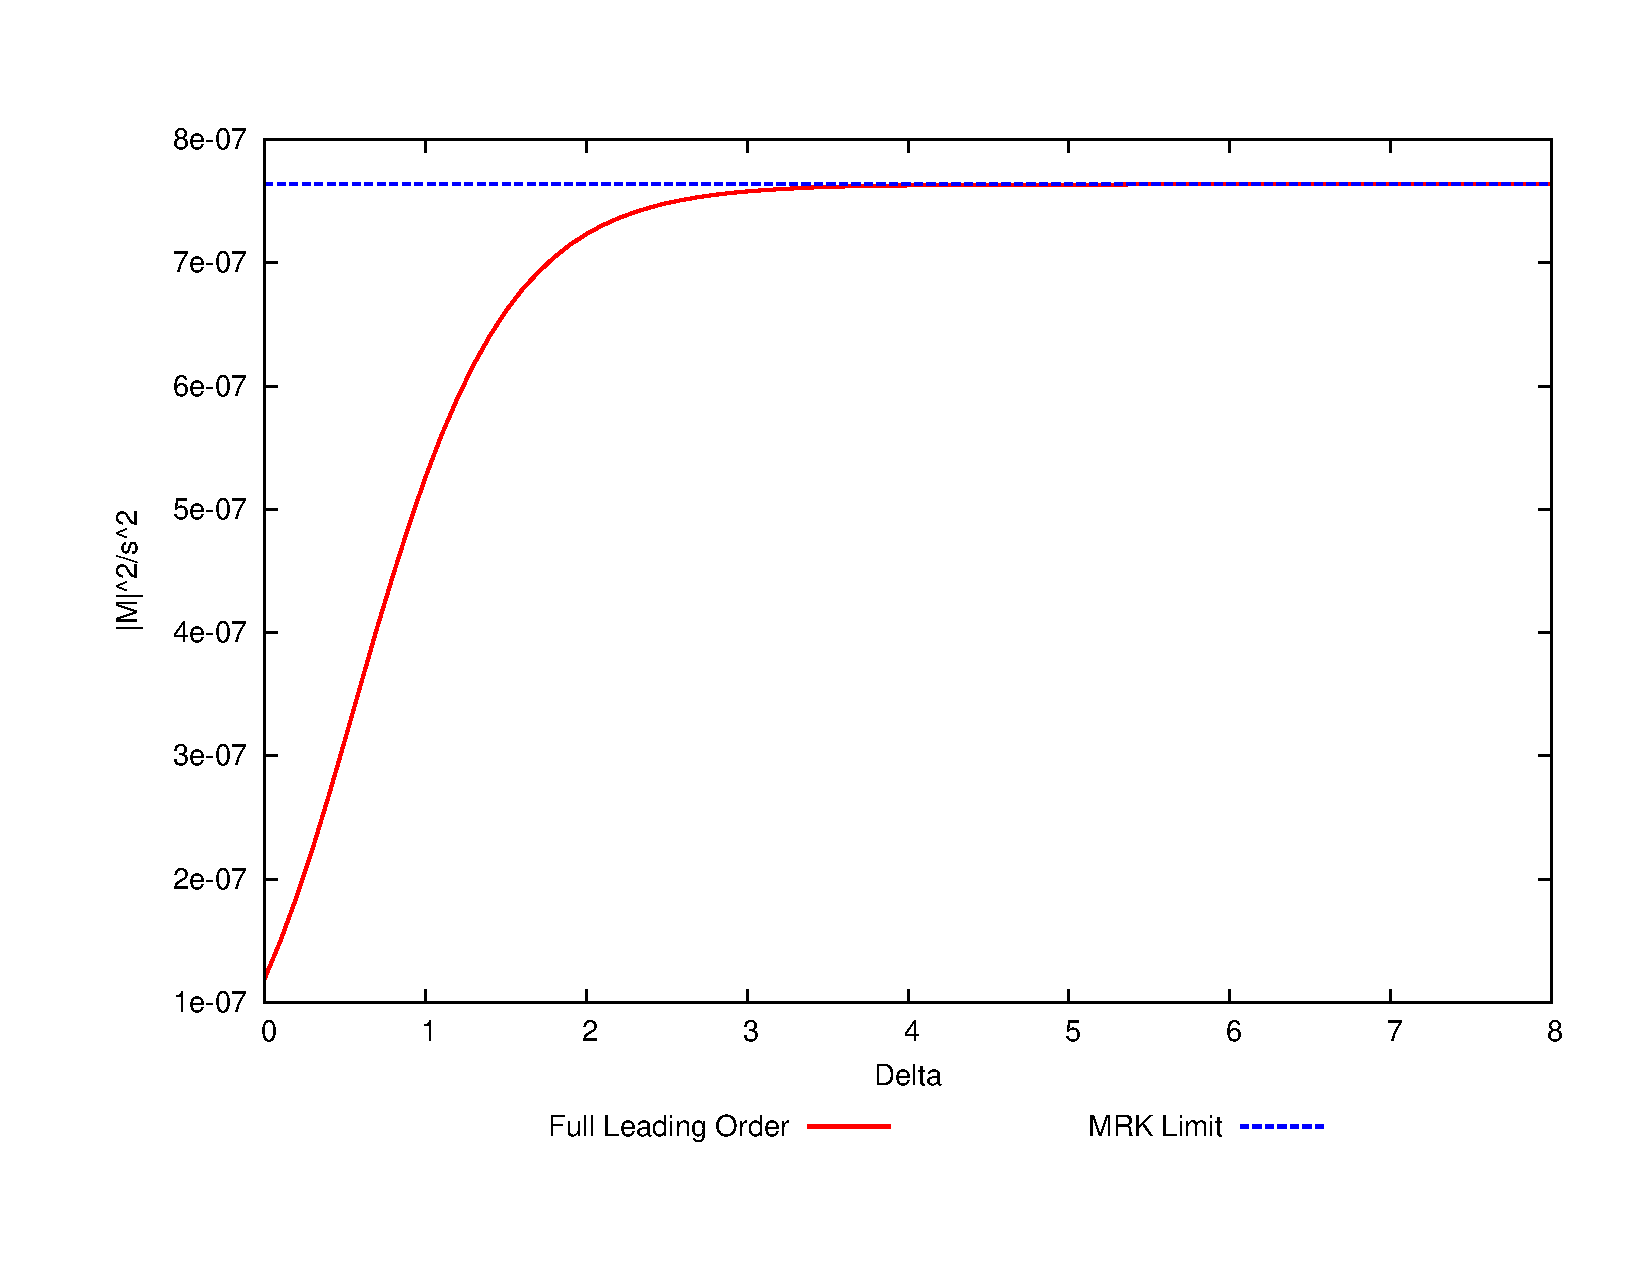
\includegraphics[scale=0.5]{Images/ud_ud_plots.pdf} 
\caption{Comparison of the full Leading Order calculation and the MRK limit of the process $ud \to ud$. A high value of $\Delta$ means that the final state particles are well-separated in rapidity.}
\label{fig:qQ_LO_MRK}
\end{figure}

For the next-to-leading order calculation, there are a number of diagrams that need to be taken into account, a selection of which are shown in figure \ref{fig:qQnlo}. If we were interested in the full NLO expression, we would have to work out the contribution from each diagram and sum them up along with the LO calculation. However, we are now interested in expressions that are relevant in the MRK regime only, so we should identify which diagrams are leading in that limit\footnote{This seems like a gauge dependent statement and indeed it is, but the argument that follows is valid for all covariant gauges, which are the only ones we will use.}; namely, diagrams that have a dependence on the rapidity gap between the two extremal partons. Therefore, we can expect that only loops that have `knowledge' of this can give rise to an expression leading in $\log(\frac{\hat{s}}{-\hat{t}})$ -- hence the terminology `Leading Logarithmic' (LL). Self-energy diagrams of the quarks, such as the one on the top right of figure \ref{fig:qQnlo}, clearly cannot be LL since the momentum of the other quark line does not enter into it and cannot influence the loop integral. A similar argument holds for the vertex correction diagrams, such as the one in the top left. For the self-energy diagram of the gluon (middle-right of the diagram) the propagators entering the loop are of the order of the transverse scale, which we keep fixed in comparison to growing $\hat{s}$ and so again cannot be leading. This leaves only the bottom two diagrams to be calculated, of which we need only do one because we can relate one to the other (up to a colour factor we can read off) via crossing symmetry. We choose to calculate the bottom-left diagram.

\begin{figure}[t]
\centering
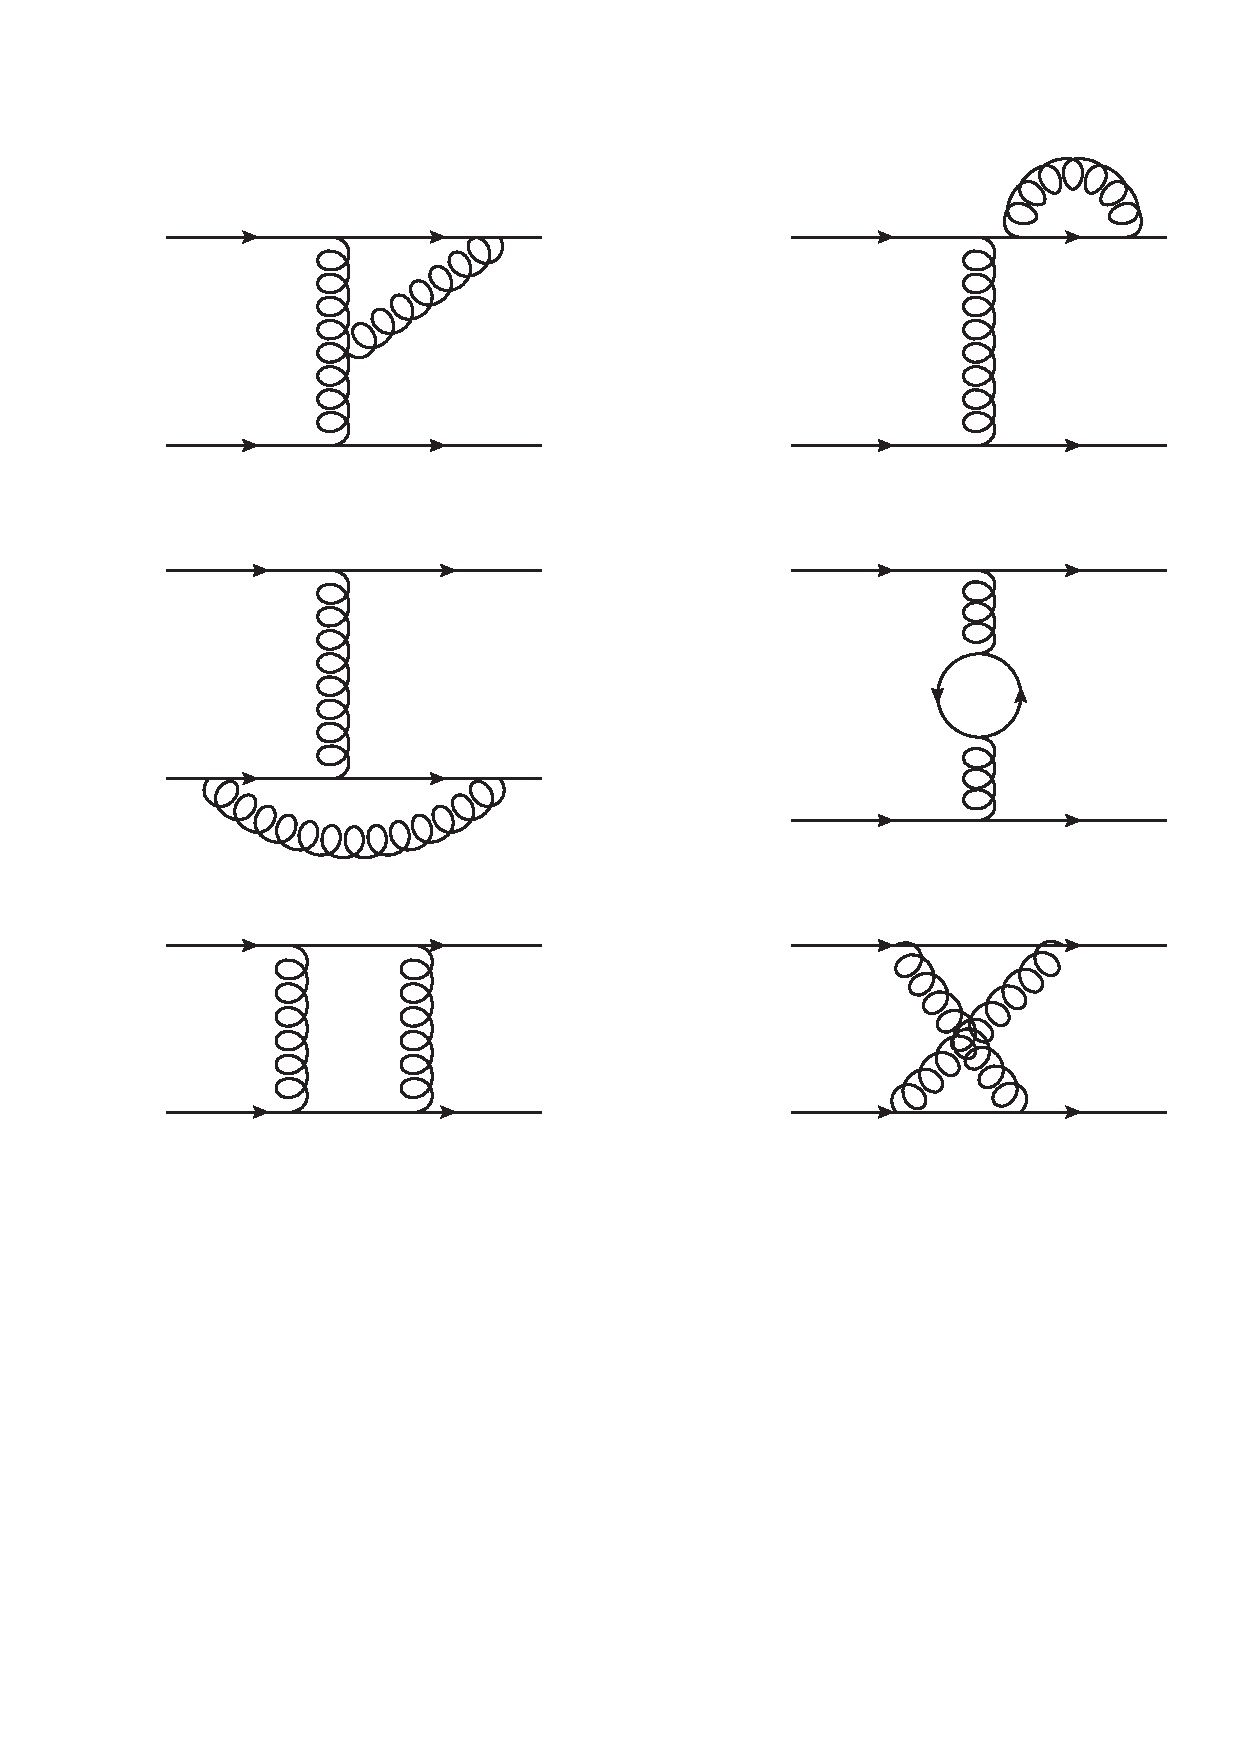
\includegraphics[scale=0.8]{Images/qQ_nlo.pdf} 
\caption{A selection of NLO diagrams for $qQ \to qQ$. We need only be interested in the bottom two.}
\label{fig:qQnlo}
\end{figure}

Feynman diagrams that involve loops are, in general, difficult to calculate. The loop momentum we need to integrate over appears in a number of fermionic and gluonic propagators, the former leading to some cumbersome spinor algebra. Fortunately, there is a way to simplify the calculation by use of the \emph{Cutkosky rules} \cite{Cutkosky1960}. We can define the matrix $S$ which encodes all possible ways a state $\ket{i}$ can evolve to a state $\ket{f}$, with elements
\begin{equation}
S_{fi} = \delta_{fi} + i(2 \pi)^4 \delta^4 \left(\sum_{i \in initial} p_i - \sum_{j \in final} p_j \right) M_{fi},
\end{equation}
where $\delta_{fi}$ represents a process where no interaction occurs and $M_{fi}$ is the scattering matrix element we have been working with before. In matrix notation, this can be written $S = \mathbb{1} + i T$ for the appropriate definition of $T$. Clearly, since the probability that an in state ends up in a particular out state, summed over all possible out states, must be unity, the matrix $S$ must be unitary, $S^\dagger S = \mathbb{1}$. This immediately leads to the non-trivial requirement
\begin{equation}
2 \hspace{1pt} \text{Im}(T) = T^\dagger T.
\end{equation}
We can project out a certain initial and final state
\begin{equation}
\begin{split}
2 \hspace{1pt} \text{Im}(T_{fi}) &= \matel{f}{T^\dagger T}{i} \\
&= \sum_{k} \matel{f}{T^\dagger}{k} \matel{k}{T}{i} \\
&= \sum_k T_{kf}^* T_{ki} \\
&= \sum_k (2 \pi)^4 \delta^4 \left(\sum_{i} p_i - \sum_{k} p_k \right) M_{kf}^*M_{ki}.
\end{split}
\end{equation}
where in the second line we have inserted a complete set of intermediate states $\ket{k}$.

This is a general statement about the full scattering amplitude. However, if we break this down into an order-by-order expression in the coupling, the statement allows one to relate diagrams at next-to-leading order (the left-hand side) to the product of other diagrams of leading order (the right-hand side). Using the Cutkosky rules, then, we can diagrammatically represent the imaginary part of the amplitude we are trying to work out as something like figure \ref{fig:cut}: we `cut' the diagram vertically, setting the quark propagators crossing the cut on-shell and treating the process as a product of two leading order processes. Algebraically, this yields

\begin{figure}[t]
\centering
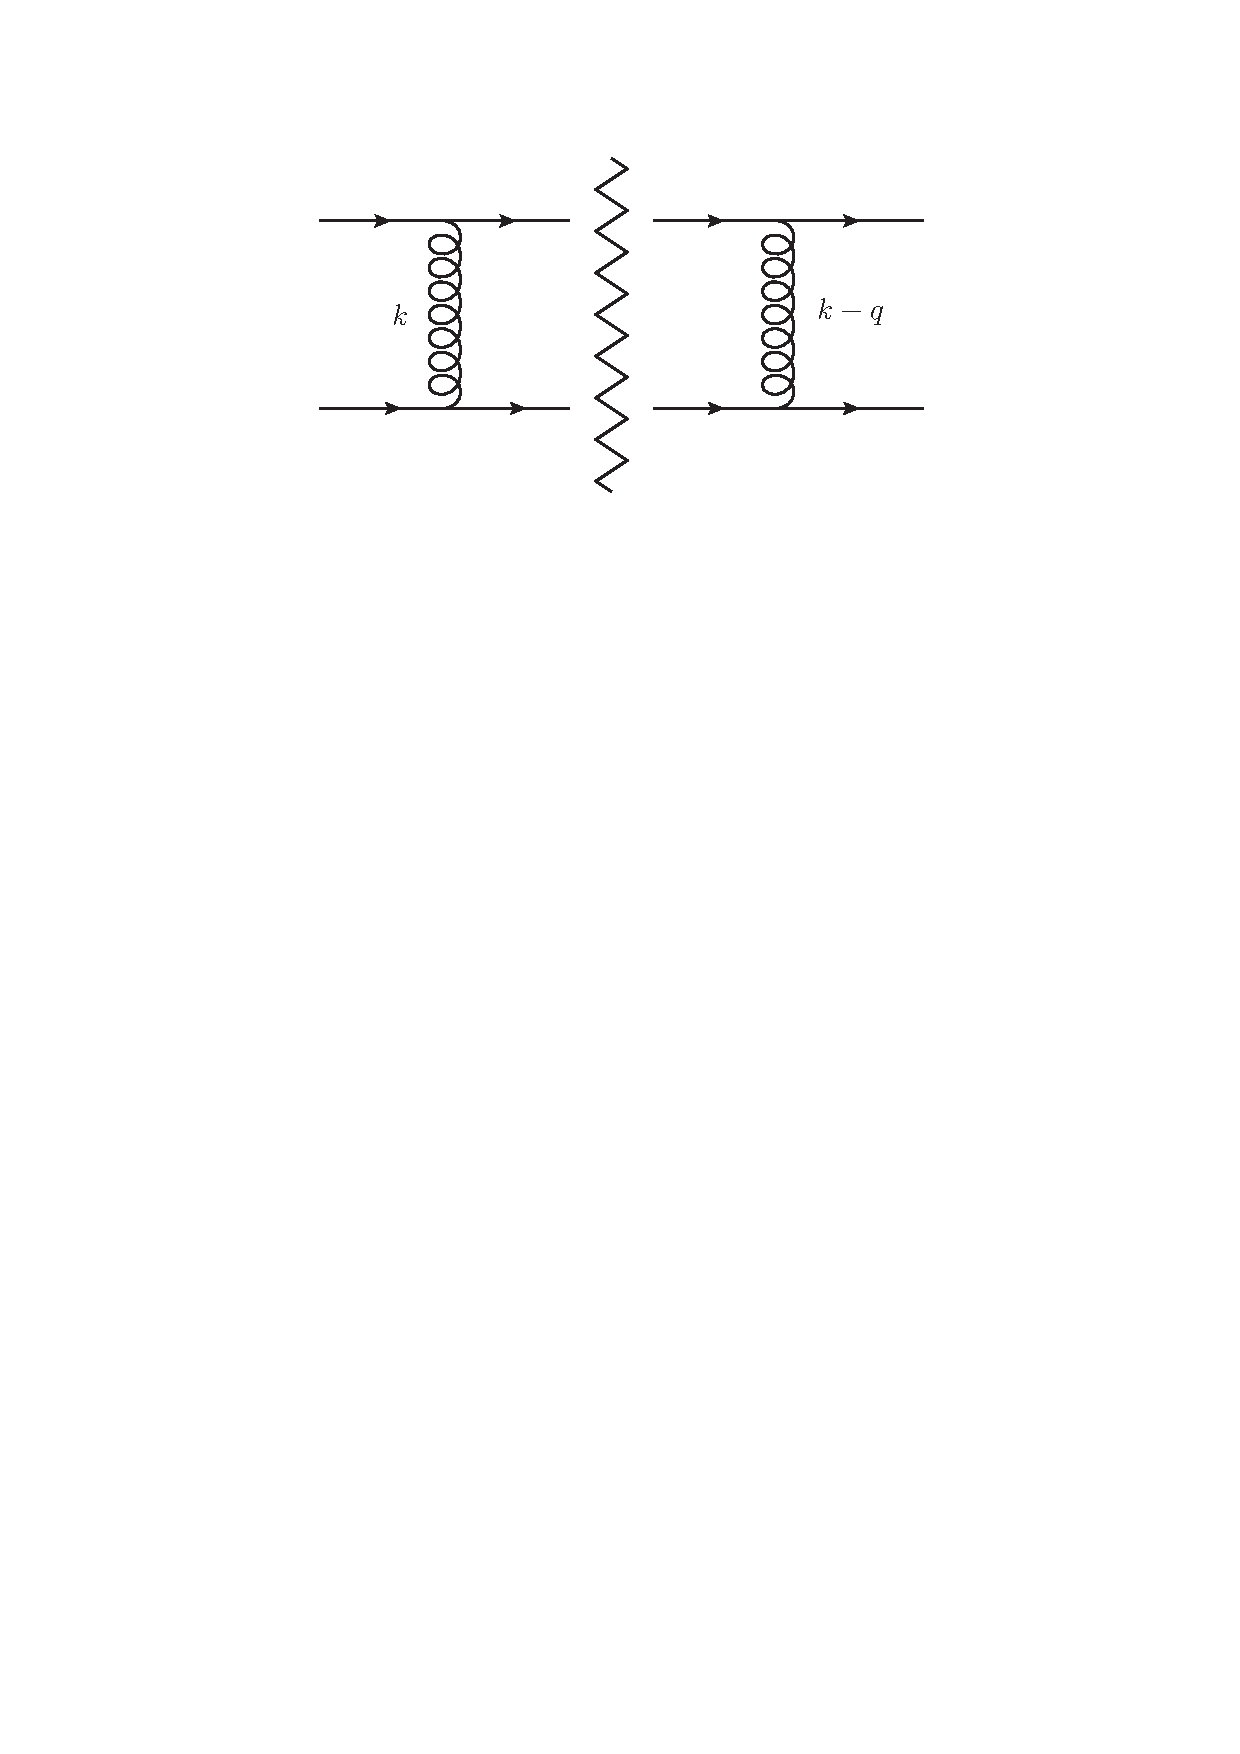
\includegraphics[scale=1]{Images/cuts.pdf} 
\caption{By `cutting' our NLO diagram like this, we can find the imaginary part of the amplitude by considering a product of LO diagrams. }
\label{fig:cut}
\end{figure}

\begin{equation}
\begin{split}
\text{Im}(M_{NLO,1}) &= \frac{1}{2} \int d(\text{phase space}) M_{LO}(k) M_{LO}^\dagger (k - q) \\
&= \frac{1}{2} \int \frac{d^4 l}{(2 \pi)^3} \frac{d^4 l'}{(2 \pi)^3} \delta(l^2) \delta(l^{'2}) (2 \pi)^4 \delta^4(p_a - p_b - l -l')  M_{LO}(k) M_{LO}^\dagger (k - q) \\
&= \frac{1}{8 \pi^2} \int d^4 k \hspace{1pt} \delta((p_a - k)^2) \delta((p_b+k)^2) M_{LO}(k) M_{LO}^\dagger (k - q).
\end{split}
\end{equation}
In the MRK limit, the leading order matrix element depended on $\hat{s}$ and $k_\perp$ as
\begin{equation}
M_{MRK} \sim g_s^2 \frac{2 \hat{s}}{|k_\perp|^2},
\end{equation}
so it would be useful to write our integration over $k^\mu$ in terms of an explicit integration over $k_\perp$. We can do this by using a Sudakov parametrisation
\begin{equation}
k^\mu = \rho p_a^\mu + \lambda p_b ^\mu + k_\perp^\mu,
\end{equation}
which allows us to switch our integration variables to $\rho, \lambda$ and $k_\perp$, with the relation $d^4k = \frac{1}{2} \hspace{1pt} \hat{s} \hspace{2pt} d \rho \hspace{2pt} d \lambda \hspace{2pt} d^2 k_\perp$. The High Energy Limit tells us that in this parametrisation, both $\rho$ and $\lambda$ are much smaller than 1. Thus
\begin{equation}
\begin{split}
\text{Im}(M_{NLO,1}) & = \frac{g_s^4 \hat{s}}{ 4 \pi^2} \int d \rho \hspace{2pt} d \lambda \hspace{2pt} d^2 k_\perp \hspace{1pt} \delta(-\hat{s}(1-\rho) \lambda + |k_\perp|^2) \\
& \times \delta(\hat{s}(1+ \lambda) \rho + |k_\perp|^2) \frac{\hat{s}}{|k_\perp|^2} \frac{\hat{s}}{|k_\perp - q_\perp|^2}  \\
& \approx \frac{g_s^4 \hat{s}^3}{ 4 \pi^2} \int d \rho \hspace{2pt} d \lambda \hspace{2pt} d^2 k_\perp \hspace{1pt} \delta(-\hat{s} \lambda + |k_\perp|^2) \delta(\hat{s} \rho + |k_\perp|^2) \frac{1}{|k_\perp|^2} \frac{1}{|k_\perp - q_\perp|^2}  \\
&= \frac{g_s^4 \hat{s}}{ 4 \pi^2} \int d \rho \hspace{2pt} d \lambda \hspace{2pt} d^2 k_\perp \hspace{1pt} \delta(-\lambda + |k_\perp|^2/\hat{s}) \delta(\rho + |k_\perp|^2/\hat{s}) \frac{1}{|k_\perp|^2} \frac{1}{|k_\perp - q_\perp|^2} \\
&= \frac{g_s^4 \hat{s}}{ 4 \pi^2} \int d^2 k_\perp \hspace{1pt}  \frac{1}{|k_\perp|^2} \frac{1}{|k_\perp - q_\perp|^2}.
\end{split}
\end{equation}
Since we are explicitly searching for terms proportional to $\Delta y = \ln \left( \frac{\hat{s}}{-\hat{t}} \right)$, then the calculation of the imaginary part immediately yields the real part, since
\begin{equation}
\ln \left( \frac{\hat{s}}{-\hat{t}} \right) = \ln \left| \frac{\hat{s}}{\hat{t}} \right| - i \pi.
\end{equation}
In effect, the pure existence of an imaginary part shows that this loop diagram contains the required logarithm. Our real part, therefore, is
\begin{equation}
\text{Re}(M_{NLO,1}) = \ln \left| \frac{\hat{s}}{\hat{t}} \right| \frac{-g_s^4 \hat{s}}{ 4 \pi^3} \int d^2 k_\perp \hspace{1pt}  \frac{1}{|k_\perp|^2} \frac{1}{|k_\perp - q_\perp|^2}.
\end{equation}
Kinematically, the other diagram we need to calculate is equivalent to this diagram under the exchange $\hat{s} \to \hat{u}$. But since in the MRK limit $\hat{s} \approx -\hat{u}$, the diagrams have the same form up to a minus sign. If there were no colour structure, the total amplitude would therefore be zero! However, we do have a colour structure which we must now treat:
\begin{equation}
\begin{split}
C_{NLO,1} - C_{NLO,2} &= t^b_{q_2 q_\alpha}t^a_{q_\alpha q_b} t^b_{q_1 q_\beta} t^a_{q_\beta q_a} -  t^a_{q_2 q_\alpha}t^b_{q_\alpha q_b} t^b_{q_1 q_\beta} t^a_{q_\beta q_a}\\
& = [t^b, t^a]_{q_2 q_b} t^b_{q_1 q_\beta} t^a_{q_\beta q_a} \\
&=\frac{if^{bac}}{2}t^c_{q_2 q_b} \left([t^b,t^a]_{q_1 q_a} + \{t^b,t^a\}_{q_1 q_a} \right) \\
&= \frac{if^{bac}}{2}t^c_{q_2 q_b} [t^b,t^a]_{q_1 q_a} \\
&= \frac{-f^{bac}f^{bad}}{2}t^c_{q_2 q_b} t^d_{q_1 q_a} \\
&= \frac{-C_A \delta^{cd}}{2}t^c_{q_2 q_b} t^d_{q_1 q_a} \\
&= \frac{-C_A}{2}C_{Tree}, \\
\end{split}
\end{equation}
where $C_A = N = 3$ is a constant associated to the $SU(3)$ group. We see that the colour factor here is simply a constant multiplied by the tree level colour factor. With a small amount of manipulation and using $\hat{t} \approx -q_\perp^2$, we can then write the leading part of the NLO amplitude as proportional to the tree-level amplitude,
\begin{equation}
M_{NLO} = M_{LO} \ln \left(\frac{\hat{s}}{-\hat{t}}\right) \hat{\alpha}(q_\perp^2),
\end{equation}
with
\begin{equation}
\label{eqn:nlocorr}
\hat{\alpha}(q_\perp^2) = \frac{C_A \alpha_s}{4 \pi^2} \int d^2 k_\perp \frac{-q_\perp^2}{k_\perp^2(k_\perp - q_\perp)^2}.
\end{equation}
This form of the amplitude clearly shows the dependence on the large logarithm. Even though $\hat{\alpha}$ contains a factor of $\alpha_s$ ,which should be small in order for our perturbation theory to make sense, the logarithm is large enough to overcome this suppression such that the product $\alpha_s \ln \left(\frac{\hat{s}}{-\hat{t}}\right)$ is of order 1. Therefore, this correction is as important as the leading order contribution and should not be ignored. In fact, terms proportional to $\alpha_s^n \ln^{n-1} \left(\frac{\hat{s}}{-\hat{t}}\right)$ continue to appear at \emph{every order} \cite{pomeronbook} and so, by the same argument, we should not ignore these contributions either. We therefore find ourselves in need of an all-order treatment of scattering amplitudes in the High Energy Limit. We will now see how the High Energy Jets (HEJ) framework achieves this. 

%\subsection{$t$-channel Pole Dominance in High Energy Scattering} \todo{Mention Regge Theory here}
%We have already seen that the full LO matrix element for $qQ \to qQ$ scattering is expressible in a form proportional to $\frac{1}{\hat{t}}$. This had to be the case since the only diagram at LO was the t-channel diagram. What we will now present is the idea that in the MRK limit, all $2 \to n$ QCD amplitudes can be expressed as proportional to one or more t-channel poles. It is important to note that this does not necessarily mean that the only contributing diagrams to a process in the MRK limit are t-channel diagrams; this is clearly a gauge-dependent statement. Rather, we will show by manipulation of the forms of amplitudes in this limit that we can \emph{factorise} amplitudes into simple functions over t-channel poles. We will then see how this factorisation allows us to capture the dominant terms in the large logarithm discussed in the previous section to all orders in perturbation theory. \\
%\\
%\todo{Need to motivate that quark-gluon and gluon-gluon 2 to 2 amps also factor into t-channel pole. Then can go onto the usual spiel about HEJ. Possibly qg calc. }

%\subsubsection{Quark/Gluon Correspondence at High Energy}
%\subsubsection{Generalisation to $2 \to n$}

\section{HEJ Amplitudes}

We have seen how taking the full MRK limit on the $qQ \to qQ$ amplitude allowed us to derive a result for the NLO virtual corrections to the process. The simplicity of that procedure should give us hope to find a way of generalising the result to obtain the virtual corrections at all orders. If we want to describe all LHC processes, however, we have a few more things to consider beforehand. Firstly, we need to account for different parton types in the incoming state. It is not clear \emph{a priori} whether $qg \to qg$ and $gg \to gg$ should behave as nicely in this limit, since the LO contribution contains more diagrams than the $t$-channel one alone. Secondly, we should account for extra final states; that is, generalise to a $2 \to n$ process. This will also be important when we want to calculate real corrections to our amplitudes, which is a subject we have not yet touched upon. We will tackle each of these concerns individually. 

\subsection{$qg \to qg$ in the High Energy Limit}

We can demonstrate how the High Energy Limit relates quarks to gluons by taking the limit on the LO $qg \to qg$ amplitude and comparing it to the $qQ \to qQ$ amplitude. There are a total of 3 diagrams we must consider, which are shown in figure \ref{fig:qg_qg_scat}. In analogy with how we calculated the $qQ \to qQ$ amplitude, we will consider the helicity configuration $q^+ g^+ \to q^+ g^+$. Since we have an external gluon now, we also have gluon polarisation vectors in our calculation. Such vectors have a gauge redundancy and so we must choose a certain gauge to work in. If we take the incoming gluon to have momentum $p_b$ and the outgoing to have momentum $p_2$, it turns out to be useful to use the following parametrisation for the vectors \cite{Dixon1996, Andersen2010}:
\begin{subequations}
\begin{align}
\varepsilon_{2 \rho}^{+*} &= \frac{\matel{2^+}{\rho}{b^+}}{\sqrt{2} \left< b 2 \right>},\\
\varepsilon_{2 \rho}^{-*} &= -\frac{\matel{b^+}{\rho}{2^+}}{\sqrt{2} \left[ b 2 \right]}, \\
\varepsilon_{b \rho}^{+} &= -\frac{\matel{2^+}{\rho}{b^+}}{\sqrt{2} \left [ 2 b \right]}, \\
\varepsilon_{b \rho}^{-} &= \frac{\matel{b^+}{\rho}{2^+}}{\sqrt{2} \left< 2 b \right>}.
\end{align}
\end{subequations}

\begin{figure}[t]
\centering
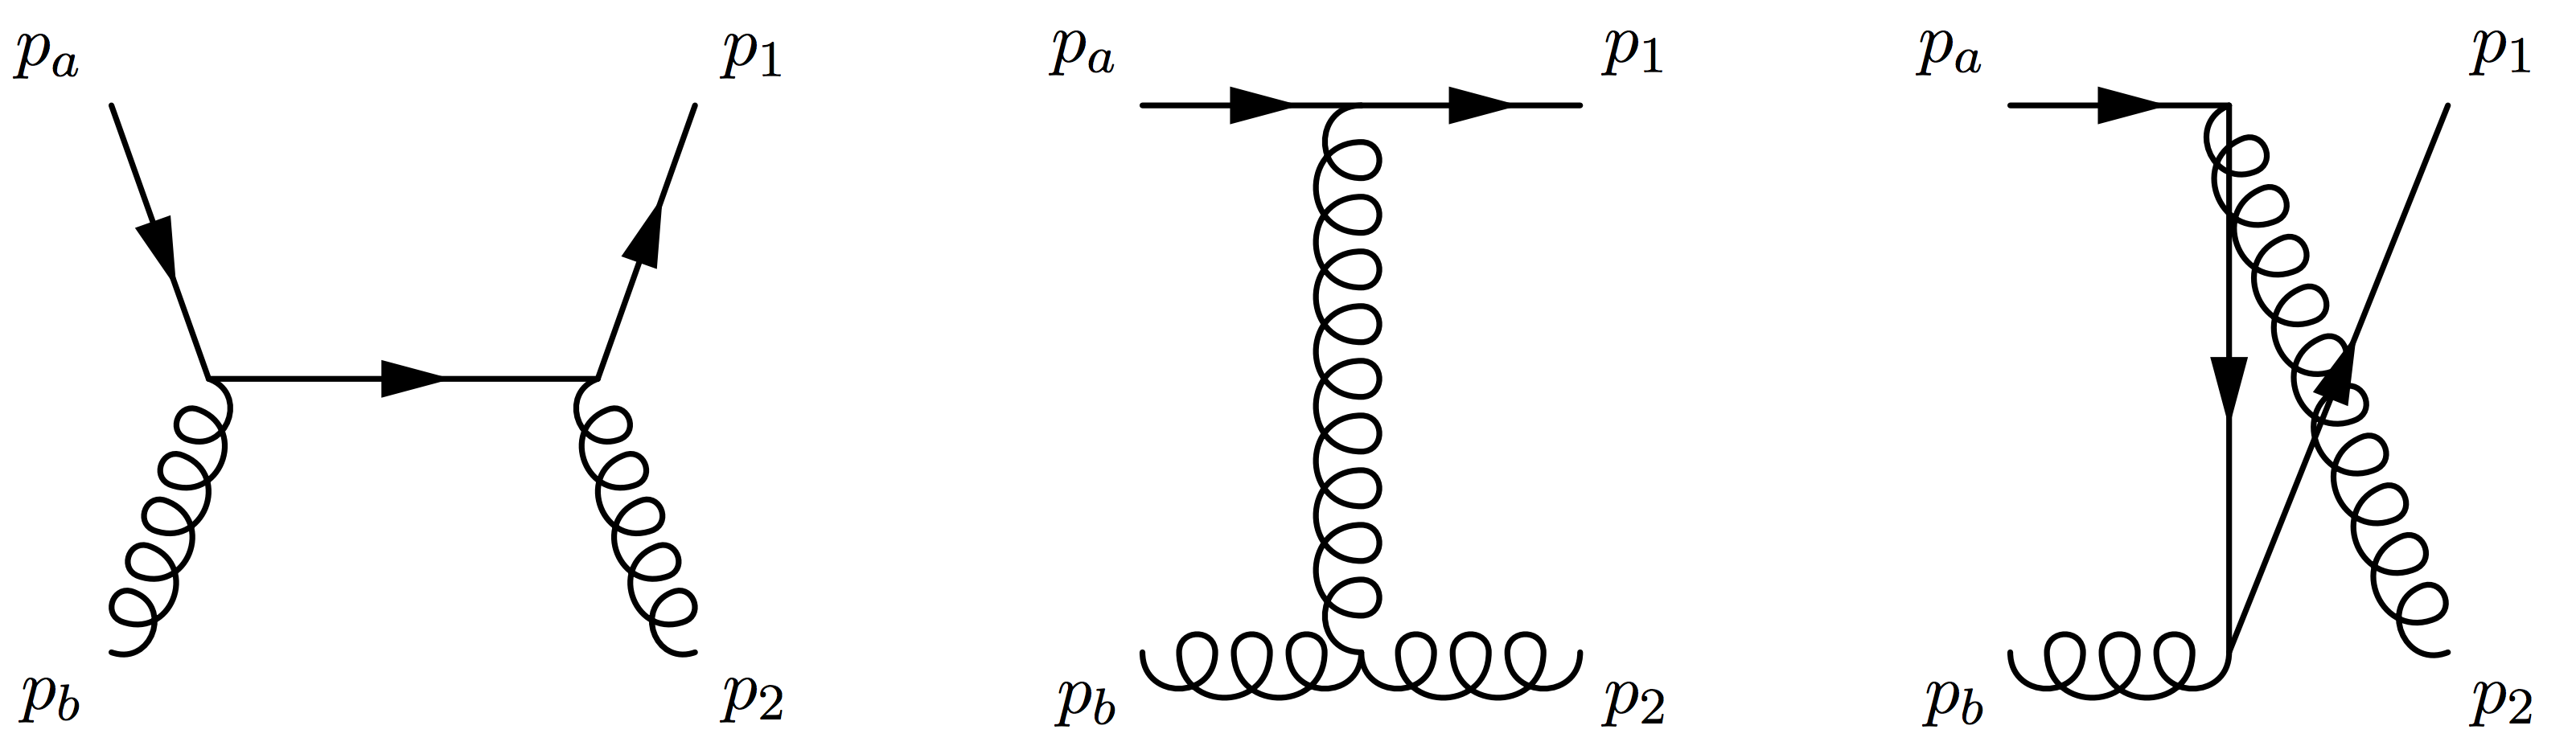
\includegraphics[scale=0.25]{Images/qg_qg_scattering.png} 
\caption{The three diagrams ($s$, $t,$ and $u$ channels) for $qg \to qg$ scattering at LO.}
\label{fig:qg_qg_scat}
\end{figure}

We conduct the calculation by moving from left to right in figure \ref{fig:qg_qg_scat} and thus begin with the $s$-channel diagram. The Feynman rules give us 
\begin{equation}
\begin{split}
M_s &= \bar{u}^+_1 (- i g_s \gamma^\nu T^2_{1q}) \left( \frac{i(\slashed{p}_a + \slashed{p}_b)}{\hat{s}}\right)(- ig_s \gamma^\mu T^b_{qa}) u_a^+ \varepsilon_{2 \nu}^{+*} \varepsilon_{b \mu}^+ \\
&= \frac{i g_s^2 T^2_{1q}T^b_{qa}}{2 \hat{s} \left<b 2 \right> [2b]} \matel{2^+}{\nu}{b^+} \matel{2^+}{\mu}{b^+} \matel{1^+}{\gamma^\nu (\slashed{p}_a + \slashed{p}_b) \gamma^\mu}{a^+} \\
&= \frac{-i g_s^2 T^2_{1q}T^b_{qa}}{\hat{s} \hat{t}} \matel{2^+}{\nu}{b^+} \matel{2^+}{\mu}{b^+} p_a^\mu \matel{1}{\nu}{a},
\end{split}
\end{equation}
where in the last line we have used the completeness relation to expand the $\slashed{p}$ terms along with some of our spinor helicity identities. The $t$-channel diagram gives
\begin{equation}
\begin{split}
M_t & = \bar{u}_1^+ (- i g_s \gamma^\mu T^g_{1a}) u_a \left(\frac{-i \eta_{\mu \nu}}{\hat{t}} \right) \\
& f^{g2b}(-g_s)(\eta^{\nu \rho}(2 p_2 - p_b)^\sigma - \eta^{\rho \sigma}(p_2 + p_b)^\nu + \eta^{\sigma \nu}(2 p_b - p_2)^\rho) \varepsilon_{2 \rho}^{+*} \varepsilon_{b \sigma}^+,
\end{split}
\end{equation}
but, since $p_{2/b}$ dotted with any of the polarisation vectors is zero and the two polarisation vectors themselves dotted together (with the chosen helicities) is also zero, we see that
\begin{equation}
M_t = 0.
\end{equation}
It is important to realise that this result only holds because of the gauge we chose; it is the final result, which is the sum of all diagrams, that is the gauge invariant quantity. Thus, though it may seem surprising at first that the $t$-channel diagram is zero given that we are trying to show that the High Energy Limit is dominated by $t$-channel poles, it is simply a consequence of our gauge choice. The final diagram is the u-channel
\begin{equation}
\begin{split}
M_u &= \bar{u}^+_1 (- i g_s \gamma^\nu T^b_{1q}) \left( \frac{i(\slashed{p}_a - \slashed{p}_2)}{\hat{u}}\right)(- ig_s \gamma^\mu T^2_{qa}) u_a^+ \varepsilon_{b \nu}^{+*} \varepsilon_{2 \mu}^+ \\
&= \frac{i g_s^2 T^b_{1q}T^2_{qa}}{2 \hat{u} \left<b 2 \right> [2b]} \matel{2^+}{\nu}{b^+} \matel{2^+}{\mu}{b^+} \matel{1^+}{\gamma^\nu (\slashed{p}_a - \slashed{p}_2) \gamma^\mu}{a^+} \\
&= \frac{-i g_s^2 T^b_{1q}T^2_{qa}}{\hat{u} \hat{t}} \matel{2^+}{\nu}{b^+} \matel{2^+}{\mu}{b^+} p_a^\mu \matel{1}{\nu}{a}.
\end{split}
\end{equation}
We see therefore that
\begin{equation}
M_{q^+g^+ \to q^+g^+}^{LO} = \frac{-i g_s^2}{\hat{t}}\matel{2^+}{\nu}{b^+} \matel{2^+}{\mu}{b^+}p_a^\mu \matel{1^+}{\nu}{a^+}\left(\frac{T^2_{1q}T^b_{qa}}{\hat{s}} + \frac{T^b_{1q}T^2_{qa}}{\hat{u}} \right).
\end{equation}
We recall now that in the High Energy Limit, $\hat{u} \approx -\hat{s}$. We can also approximate that
\begin{equation}
\matel{2^+}{\mu}{b^+} p_a^\mu \approx 2 p_b \cdot p_a  = \hat{s}.
\end{equation}
Applying the limit to our result we see that 
\begin{equation}
M_{q^+g^+ \to q^+g^+}^{LO, HE} = \frac{g_s^2 f^{2bc}T^c_{1a}}{\hat{t}}\matel{2^+}{\nu}{b^+} \matel{1^+}{\nu}{a^+},
\end{equation}
and therefore the amplitude is expressible as proportional to a $t$-channel pole. Furthermore, by taking the absolute square of this along with the colour sum, we find that
\begin{equation}
|M_{q^+g^+ \to q^+g^+}^{LO, HE}|^2 = \frac{C_A}{C_F} |M_{q^+Q^+ \to q^+Q^+}^{LO, HE}|^2,
\end{equation}
where, for the $SU(3)$ group, we have $C_A = 3$ and $C_F = \frac{4}{3}$. We therefore have that the High Energy Limit relates quarks to gluons in a very simple way: namely, via the multiplication of a colour factor. We find that this result holds for the other `helicity conserving' amplitudes (i.e., the amplitudes where both the quark and gluon do not flip helicities in the scattering) and that the `helicity non-conserving' amplitudes are identically zero, so we can in fact generalise this to
\begin{equation}
|M_{qg \to qg}^{LO, HE}|^2 = \frac{C_A}{C_F} |M_{qQ \to qQ}^{LO, HE}|^2.
\end{equation}
Of course, this equality only holds in the full High Energy Limit. However, we can improve this slightly by instead multiplying by a momentum-dependent colour factor. Such a factor was found in \cite{Andersen2010} and named the \emph{Colour Acceleration Multiplier}:
\begin{equation}
\tilde{C}_A = \frac{1}{2} \left(C_A - \frac{1}{C_A} \right) \left(\frac{p_b^-}{p_2^-} + \frac{p_2^-}{p_b^-} \right).
\label{eqn:CAM}
\end{equation}
It is clear that this tends to $C_A$ in the limit where $p_2^- \sim p_b^-$. Using this multiplication factor instead of the straight $C_A$ allows for the approximation to be more accurate away from the strict High Energy Limit and we therefore employ it in the rest of this thesis (and, indeed, in the HEJ formalism itself). 

\subsection{Regge Theory and the Connection to High Energy $2 \to n$ Amplitudes} 

It is instructive here to take a short detour into the realm of Regge theory, which relates to properties of general scattering processes. In particular, before the advent of a full QCD theory, the relativistic form of Regge theory allowed for some predictions to be made about strongly interacting particles. More specifically, it predicts that in the High Energy Limit the amplitude of a given scattering process should behave as the Mandelstam variable $s$ raised to the power of the spin of the particle exchanged in the $t$-channel (denoted by $\alpha(t)$),
\begin{equation}
M_{Regge} \sim s^{\alpha(t)}.
\end{equation}
A more complete description of the history of the use of Regge theory applied to strong dynamics can be found in \cite{pomeronbook}. For our purposes, we need only remark that the expression generalises if there is instead a `chain' of exchanged particles in the $t$-channel such as that shown in figure \ref{fig:mrk}, and we describe such a configuration as `Multi-Regge Kinematical': 
\begin{equation}
M_{Multi-Regge} \sim s_{12}^{\alpha(t_1)} s_{23}^{\alpha(t_2)} \cdots s_{n-1,n}^{\alpha(t_{n-1})}.
\end{equation}
\begin{figure}[t]
\centering
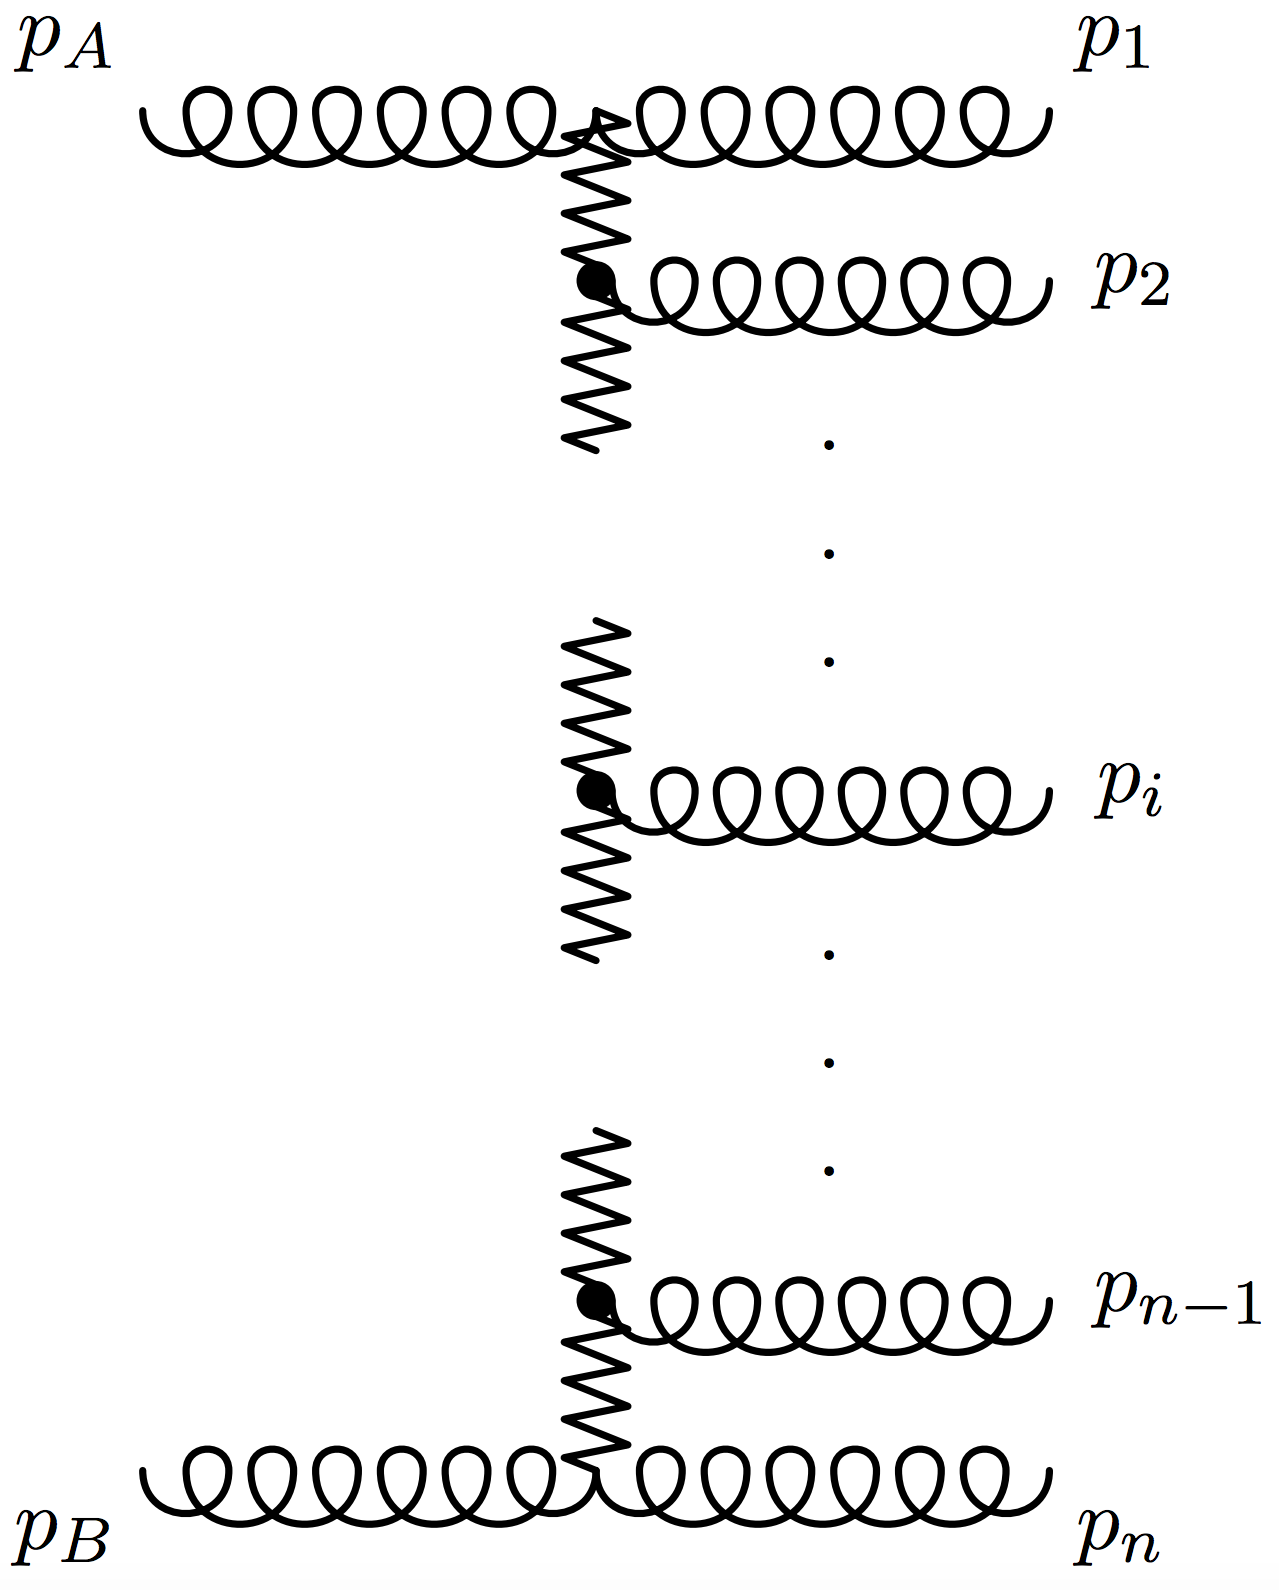
\includegraphics[scale=0.3]{Images/MRK_diagram.png} 
\caption{A schematic representation of an example MRK amplitude. Taken from \cite{Andersen2009a}.}
\label{fig:mrk}
\end{figure}

We have already seen in $qQ \to qQ$ scattering that the amplitude did indeed behave as $s^1$ in the MRK limit. Since our only two choices of particles involved in $t$-channel exchange are the spin-one gluon and the spin-half quark, clearly all leading amplitudes in this limit must only have gluons exchanged. The only thing that can be emitted from a t-channel gluon is another gluon (any quark must be accompanied by an anti-quark, with an intermediate t-channel quark propagator) and so we need only consider extra gluon emissions from our base $2 \to 2$ processes to capture all the leading contributions. Such configurations are also referred to as `Fadin-Kuraev-Lipatov' or simply FKL configurations \cite{Kuraev1976}, named after the three scientists who developed the formalism. Use of this fact and the study of amplitudes within the strict MRK limit \cite{DelDuca1995, Andersen2009a} show that the analytical form of the amplitude is
\begin{equation}
|M^{MRK}_{f_1 f_2 \to f_1 g ... g f_2}|^2 = \left(\frac{4 \hat{s}^2}{N_c^2 - 1} \right) \frac{g^2 C_{f_1}}{|p_{1 \perp}|^2} \left(\prod_{i = 2}^{n-1} \frac{4 g^2 C_A}{|p_{i \perp}|^2} \right)  \frac{g^2 C_{f_2}}{|p_{n \perp}|^2} ,
\end{equation}
where $C_{f_1}, C_{f_2}$ are $C_F, C_A $ depending on whether the incoming particles are quarks or gluons respectively. However, as we saw when we took the explicit limit of the $qQ \to qQ$ amplitude, this limit is only physically useful for a small amount of the available phase space that the LHC explores. On the other hand, the analytic expression is remarkably simple and at high gluon multiplicities it is much more practical to calculate than a full LO expression. Ideally, we would like to have something that bridges the gap between these two points; an expression that follows more closely the full LO matrix element in the LHC phase space whilst at the same time being simple enough such that we can evaluate it for processes with large numbers of final state gluons. The formulation of such amplitudes is one of the cornerstones of HEJ. 

\subsection{$qQ \to qgQ$ in the High Energy Limit}

A good basis for finding a simple formulation for gluon emission away from the full MRK limit is to consider an extra emission in our $qQ$ scattering process, since the only possible choice there is $qQ \to qgQ$. There are a total of five diagrams for this, which are shown in \ref{fig:qQqgQ}. Before we begin the calculation, let us first take a detour to discuss the \emph{Eikonal Approximation}.

\begin{figure}[t]
\centering
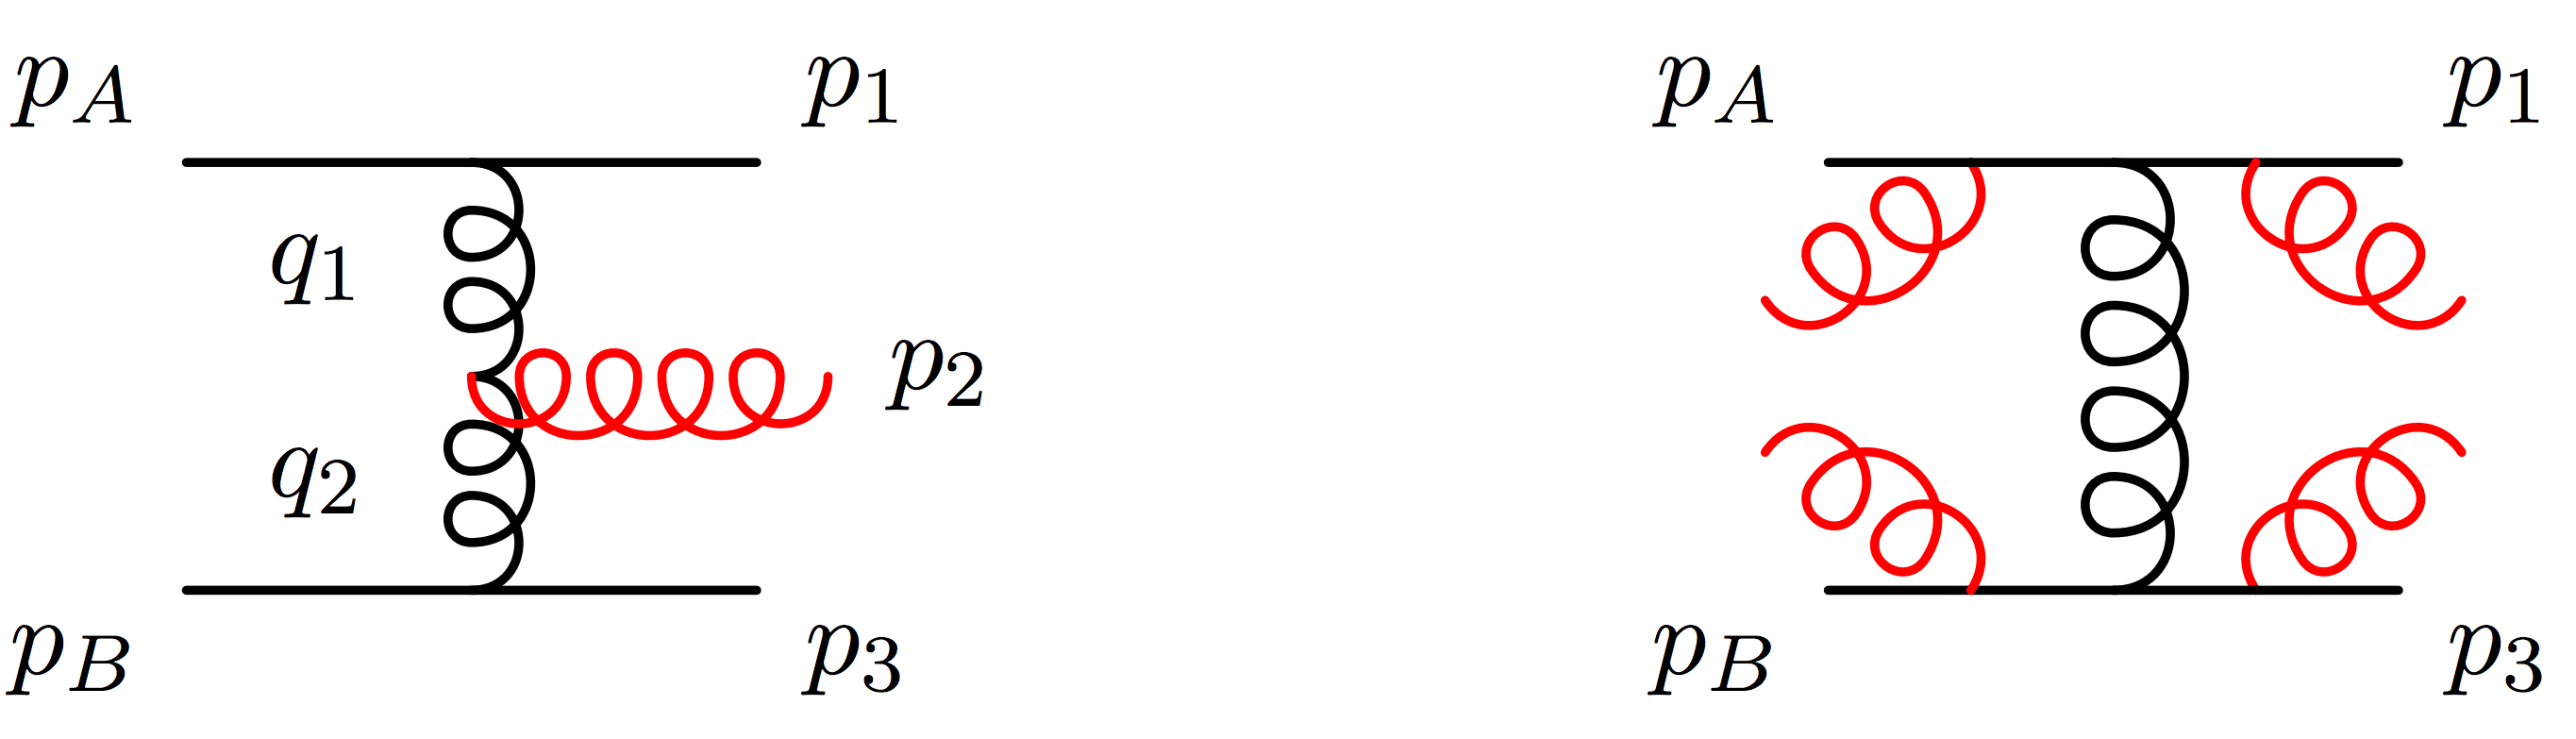
\includegraphics[scale=0.3]{Images/gluon_emission.png} 
\caption{The five possibilities for an extra gluon emission. The diagram on the right-hand side should be seen as four separate diagrams. Taken from \cite{Andersen2009a}.}
\label{fig:qQqgQ}
\end{figure}

The Eikonal Approximation is a way of simplifying the structure of vertex functions in the limit where one of the momenta entering the vertex becomes very small. We will show that this approximation is also valid for situations where a momentum is not small in an absolute sense but small compared to other momenta in the problem. This is best seen by considering an example. Take a quark-quark-gluon vertex such as the one shown in figure \ref{fig:eikonal}, where the quark line connects to a larger diagram on the left-hand side and the gluon is a final state particle. The Feynman rules for such a part of the diagram give an expression that includes the term $\bar{u}(p) \gamma^\mu (\slashed{p} + \slashed{k})/(p+k)^2$. If we imagine that our quark is not deflected much by this emission, then we can take the limit $k \ll p$. This gives
\begin{equation}
\begin{split}
\frac{\bar{u}(p) \gamma^\mu (\slashed{p}+\slashed{k})}{(p+k)^2} &\approx \frac{\bar{u}(p)\gamma^\mu \slashed{p}}{2 p \cdot k} \\
&= \frac{\bar{u}(p)\gamma^\mu \gamma^\alpha p_\alpha}{2 p \cdot k} \\
&=  \frac{\bar{u}(p)(2 \eta^{\mu \alpha} - \gamma^\alpha \gamma^\mu) p_\alpha}{2 p \cdot k} \\
&= \bar{u}(p) \frac{p^\mu}{p \cdot k},
\end{split}
\end{equation}
\begin{figure}[t]
\centering
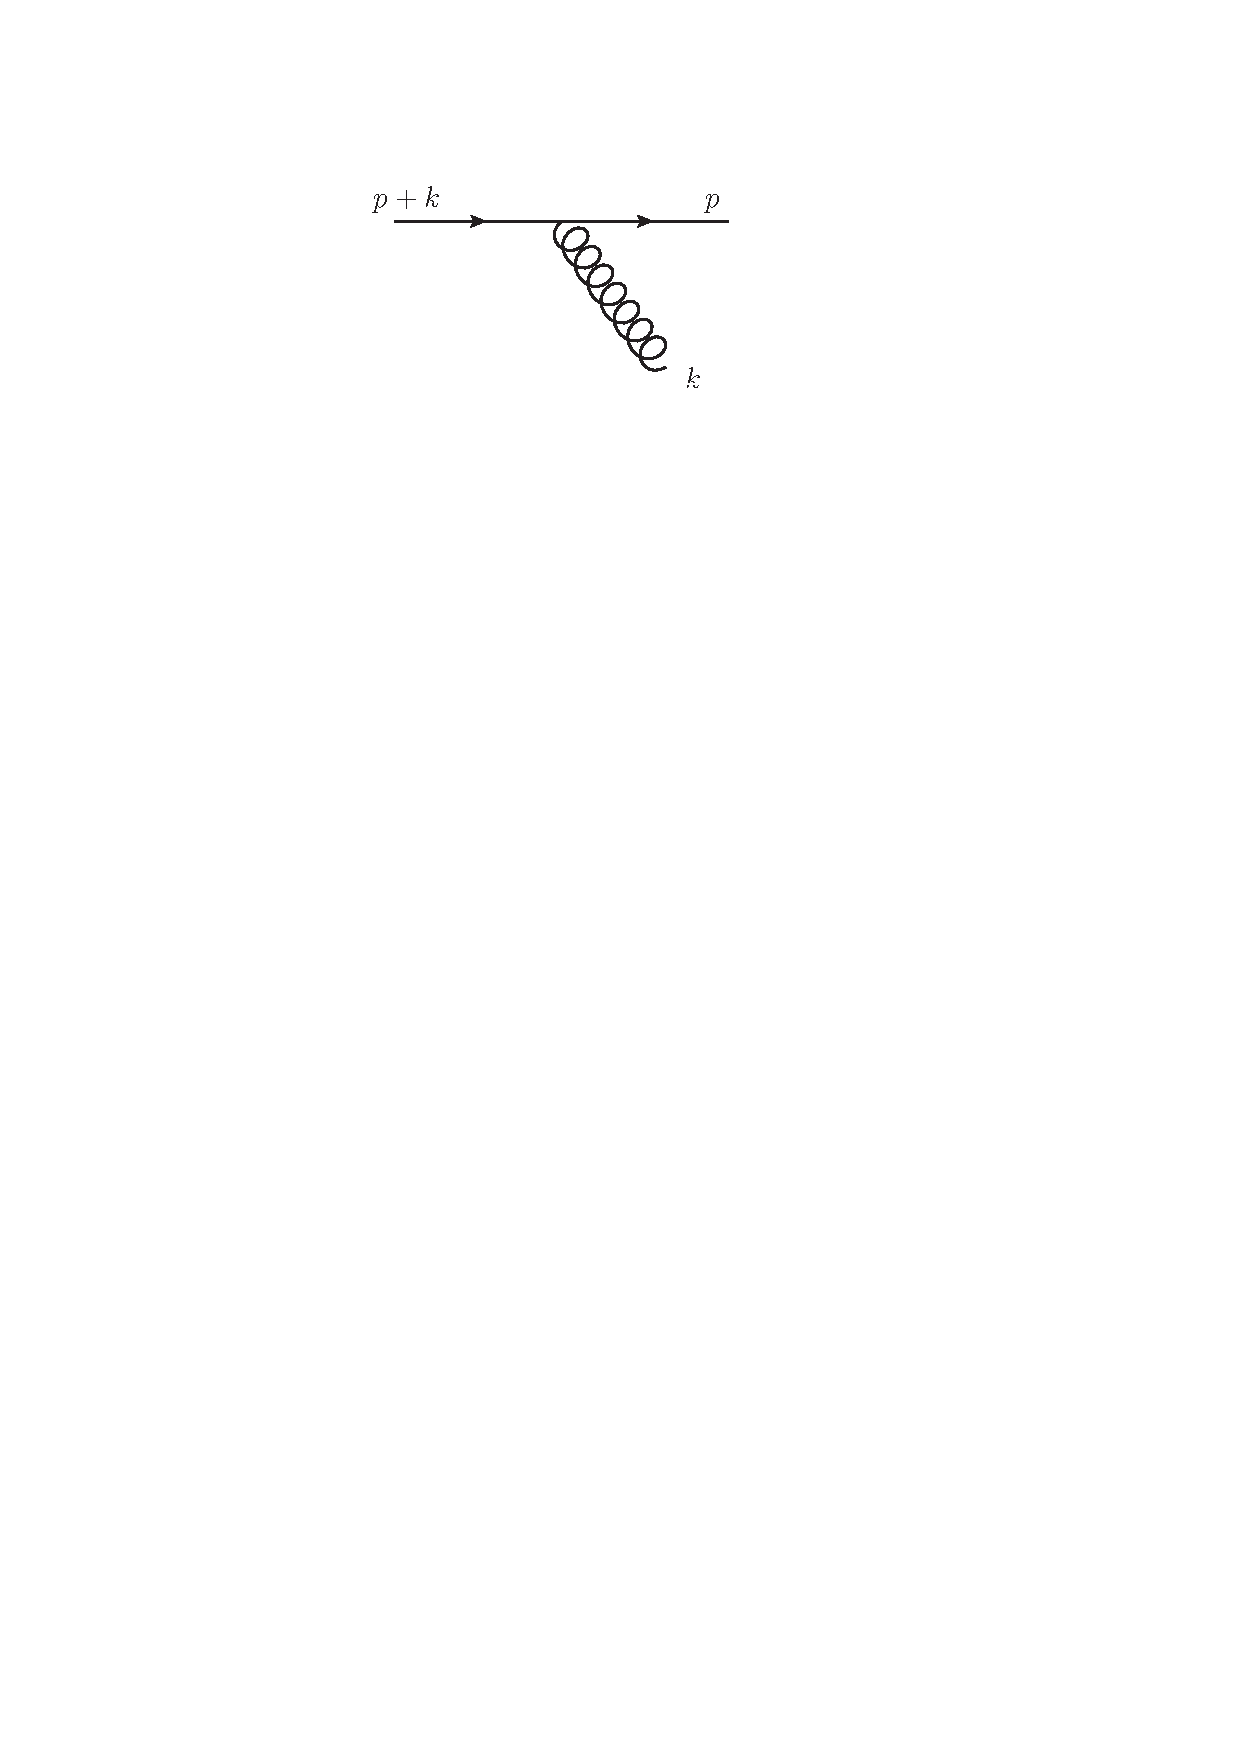
\includegraphics[scale=1.5]{Images/eikonal.pdf} 
\caption{The emission of a gluon from a quark line. By taking the limit $k \ll p$, we obtain the Eikonal rule.}
\label{fig:eikonal}
\end{figure}

where in the last line we have used $\bar{u}(p) \slashed{p} = 0$ by virtue of the Dirac equation. A similar result holds if we replace our quarks with gluons as well, so the approximation is `blind' to the spin of the particle emitting the gluon, an effect that allows us to very easily relate quarks and gluons in the High Energy Limit even as the final state multiplicity increases. We then see that the leading terms in the High Energy limit are equivalent to the leading terms in the Eikonal Limit. 

Using this approximation, we can calculate the four diagrams with a gluon emitted from the extremal legs straightforwardly. The result of adding all these contributions together gives
\begin{equation}
M_{eik} = M_{qQ \to qQ} (i g_s) \varepsilon_\rho^* \left(C_1\frac{p_1^\rho}{p_1 \cdot p_2} - C_2\frac{p_a^\rho}{p_a \cdot p_2} + C_3\frac{p_3^\rho}{p_3 \cdot p_2} - C_4\frac{p_b^\rho}{p_b \cdot p_2}  \right).
\end{equation}
The form of the approximation makes it clear that the (kinematic part of the) amplitude must be proportional to the $qQ \to qQ$ amplitude. The last diagram, however, involves emission from the $t$-channel exchanged gluon and so it is not clear if this will also be simply proportional to the $qQ \to qQ$ result. The relevant part of this diagram is
\begin{equation}
M_{3g} \sim \matel{1}{\mu}{a} (- g_s)(\eta^{\mu \rho}(q_1 + p_2)^\nu + \eta^{\rho \nu}(-p_2 + q_2)^\mu + \eta^{\nu \mu}(-q_2 - q_1)^\rho) \matel{3}{\nu}{b} \varepsilon^*_\rho,
\end{equation}
where $q_1 = p_a - p_1$ and $q_2 = p_a - p_1 -p_2 = p_3 - p_b$. In the High Energy Limit, we have already discussed how the extremal partons in the amplitude have momenta similar to the incoming particles; in other words, $p_1 \sim p_a$ and $p_3 \sim p_b$. In turn, this means that $\matel{1}{\mu}{a} \sim 2p_a^\mu$ and $\matel{3}{\nu}{b} \sim 2p_b^\nu$. Applying these approximations to our amplitude, we find 
\begin{equation}
\begin{split}
M_{3g} &\sim (- g_s)\varepsilon_\rho^*(2p_b^\rho(s_{1a} + 2 s_{a2}) - 2 p_a^\rho (s_{3b} + 2 s_{2b}) + 2 \hat{s} (-q_2 - q_1)^\rho) \\
& \approx (- 2 \hat{s}  g_s)\varepsilon_\rho^*  \left (2p_b^\rho \frac{s_{a2}}{\hat{s}} - 2 p_a^\rho \frac{s_{2b}}{\hat{s}} + (q_1 + q_2)^\rho \right),
\end{split}
\end{equation}
since $s_{1a} \ll s_{2a}$ and $s_{3b} \ll s_{b2}$. Reinstating the factors from the rest of the diagram and rewriting the $2 \hat{s}$ we factorised outside as $\matel{1}{\mu}{a} \matel{3}{\mu}{b}$, then
\begin{equation}
M_{3g} = M_{qQ \to qQ} C_t(-g_s)\varepsilon_\rho^*  \left (2p_b^\rho \frac{s_{a2}}{\hat{s}} - 2 p_a^\rho \frac{s_{2b}}{\hat{s}} + (q_1 + q_2)^\rho \right),
\end{equation}
and therefore the $qQ \to qQ$ amplitude does indeed completely factor out in this limit. We now turn our attention to the colour factors
\begin{equation}
\begin{split}
C_1 - C_2 &= t^g_{b2} t^e_{1q} t^g_{qa} - t^g_{b2} t^g_{1q} t^e_{qa} \\
&=  if^{gec}t^c_{a1}t^g_{b2} \\
&= -i C_t,
\end{split}
\end{equation}
and similarly $C_3 - C_4 = iC_t$. The sum of all the diagrams is then proportional to the same colour factor and to the $qQ \to qQ$ amplitude. Putting everything together, we can then write
\begin{equation}
M_{qQ \to qgQ} = g_s^3 C_t \varepsilon^*_\rho \frac{\matel{1}{\mu}{a} \matel{3}{\mu}{b}}{q_1^2 q_2^2} V^\rho (q_1, q_2),
\end{equation}
where
\begin{equation}
V^\rho(q_1, q_2) = -(q_1 + q_2)^\rho + p_a^\rho \left( \frac{q_1^2}{p_2 \cdot p_a} + 2 \frac{p_2 \cdot p_b}{p_a \cdot p_b}\right) -  p_b^\rho \left( \frac{q_2^2}{p_2 \cdot p_b} + 2 \frac{p_2 \cdot p_a}{p_a \cdot p_b}\right)
\label{eqn:lipatov}
\end{equation}
is an \emph{effective} or \emph{Lipatov} vertex describing the emission of a gluon. Since this vertex was derived by approximating $p_a$ with $p_1$ and $p_b$ with $p_3$, we can symmetrise this vertex in these momenta to `undo' this approximation somewhat\footnote{This symmetrised version is used in practice but adds nothing to the discussion here.}. The important point is that we can now construct an amplitude with any number of extra gluons by simply inserting the relevant number of Lipatov vertices. As previously discussed, the difference between amplitudes with initial state quarks and amplitudes with initial state gluons is an overall colour factor, so a general $2 \to n$ amplitude takes the form
\begin{equation}
\begin{split}
|\bar{M}^t_{f_1 f_2 \to f_1 g ... g f_2}|^2 &= \frac{1}{4 (N_C^2 - 1)} ||S_{f_1 f_2 \to f_1 f_2} ||^2 \left(g_s^2 C_{f_1} \frac{1}{\hat{t}_1} \right) \left(g_s^2 C_{f_2} \frac{1}{\hat{t}_{n-1}} \right) \\
& \prod_{i=1}^{n-2} \left(\frac{-g_s^2 C_{A}}{\hat{t}_i \hat{t}_{i+1}} V^\mu (q_i, q_{i+1}) V_\mu (q_i, q_{i+1})  \right),
 \end{split}
\end{equation}
where we have introduced the notation $||S_{f_1 f_2 \to f_1 f_2}||^2$ to represent the sum over helicities of the modulus squared of the contraction of currents that appears at tree-level. We have also used the result $\sum_{pol} \varepsilon_{\mu} \varepsilon_{\nu}^* \to -\eta_{\mu \nu}$ to contract the Lipatov vertex. In the full MRK limit, this is proportional to $\hat{s}^2$ as we saw earlier, but we are able to keep more information about the process by keeping the full dependence like this (for example, we will reproduce \emph{exactly} the full LO $qQ \to qQ$ calculation in this manner, not just the MRK limit thereof). We can represent a HEJ amplitude pictorially as shown in figure \ref{fig:hejamp}. We see clearly how this expression has the simplicity of the full MRK expression whilst at the same time being more flexible, as it is able to describe better the behaviour of the matrix element away from this limit. %\todo{backslash l for closer together vertical lines}

\begin{figure}[t]
\centering
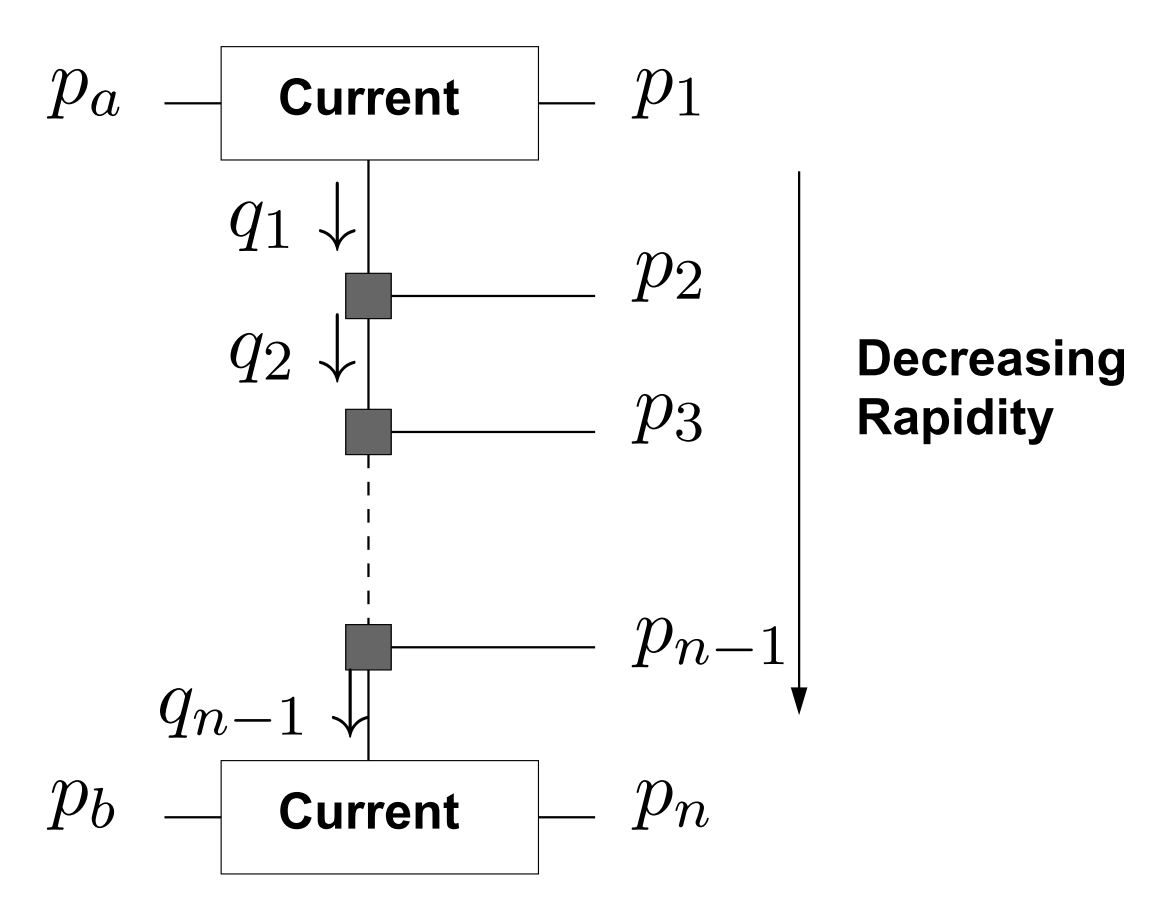
\includegraphics[scale=0.35]{Images/hej_amp.png} 
\caption{A schematic view of a HEJ amplitude. Taken from \cite{Andersen2011a}.}
\label{fig:hejamp}
\end{figure}

\section{Resummation Technique}

So far, we have derived an approximation to the LO matrix element for a certain subset of $2 \to n$ processes. We will now show that the form of this approximation allows for the inclusion of the High Energy leading logarithmic terms of the amplitude \emph{to all orders in perturbation theory}. 

\subsection{Lipatov Ansatz}

Earlier, we saw explicitly that the Leading Logarithmic contribution to the NLO correction for $qQ \to qQ$ scattering was given by multiplying the LO result by a logarithm and a factor as given by equation \ref{eqn:nlocorr}. One of the postulates of the \emph{Lipatov Ansatz} is that this result exponentiates, such that the virtual corrections to this process to all orders are given by
\begin{equation}
M_{qQ \to qQ}^{LO + virt} = M_{qQ \to qQ}^{LO} \times \exp \left[\hat{\alpha}(q_\perp) \Delta y \right],
\end{equation}
where we have related $\Delta y$ to the logarithm as explained at the beginning of section 2.1. The ansatz then goes further to say that this exponentiation holds in the MRK limit for any number of $t$-channel propagators present at the leading order, such that the virtual corrections are obtained by making the substitution
\begin{equation}
\frac{1}{\hat{t}_i} \to \frac{1}{\hat{t}_i} \exp \left[\hat{\alpha}(q_{i,\perp}) \Delta y_{i,i+1} \right].
\label{eqn:lipansatz}
\end{equation}
In the appropriate limit, this ansatz has been proved to the sub-leading level \cite{Bogdan2006,Fadin2005,Fadin2004,Fadin2006}. However, by inspection of the $\hat{\alpha}$ function given in equation \ref{eqn:nlocorr}, we see that it is clearly divergent; for small values of $k_\perp$ in the integration region, the integrand tends to infinity. Such a divergence is called an \emph{infrared divergence} and is a common problem in particle physics amplitudes involving massless particles. The problem arises because virtual corrections are not the only corrections to an amplitude we need to consider. We can also have the case where a real emission has taken place but at an energy scale small enough that only a detector with infinite resolution could have detected it. Since such a detector cannot exist, there is no way of differentiating between a `pure' $qQ \to qQ$ scattering and another one accompanied by the emission of a low energy (or `soft') gluon. Such contributions are also divergent, but in such a way that when combined with the divergence in the virtual corrections, the divergences cancel. We will show precisely how this happens in the next part. For now, we choose to use the technique of \emph{dimensional regularisation} to rewrite our $\hat{\alpha}$ function in a more convenient way that makes the divergence clear. The formalism works by extending the dimensionality of the two-dimensional perpendicular component integral to $2 + 2 \varepsilon$ dimensions. This will allow us to write the result as an expansion in $\varepsilon$, which will manifest our divergence as a term proportional to $\varepsilon^{-1}$. We must eventually take the limit $\varepsilon \to 0$, but we will see how this prescription allows us to remove the divergences from our theory in a neat and systematic way before we do so. A further note is that this dimensional shift also slightly alters the overall energy dimension of the integral and so we must introduce a scale $\mu$ to absorb this effect. The upshot is that we perform the integral in this convention and end up with %\todo{I should do this for my own sanity and understanding}
\begin{equation}
\hat{\alpha}(q_{i \perp}, \varepsilon) = - g^2 C_A \frac{\Gamma(1 - \varepsilon)}{(4 \pi)^{2 + \varepsilon}} \frac{2}{\varepsilon} \left(\frac{|q_{i \perp}|^2}{\mu^2} \right)^\varepsilon.
\end{equation}

\subsection{Combining Real and Virtual Corrections at All Orders}

As already discussed, the real correction to the amplitude occurs when the momentum of an outgoing gluon becomes very small. Since the emissions are controlled entirely by the effective vertex, we then need to find the limit of the function as the momenta becomes small. It is a simple exercise to show that, if we denote the emitted momentum by $p_2$ as in figure \ref{fig:realcorrection}, the soft limit is
\begin{equation}
\lim_{p_2 \to 0} \frac{-V(q_1, q_2) \cdot V(q_1,q_2)}{\hat{t}_1 \hat{t}_2} = \frac{4}{|p_{2 \perp}|^2}.
\end{equation}
\begin{figure}[t]
\centering
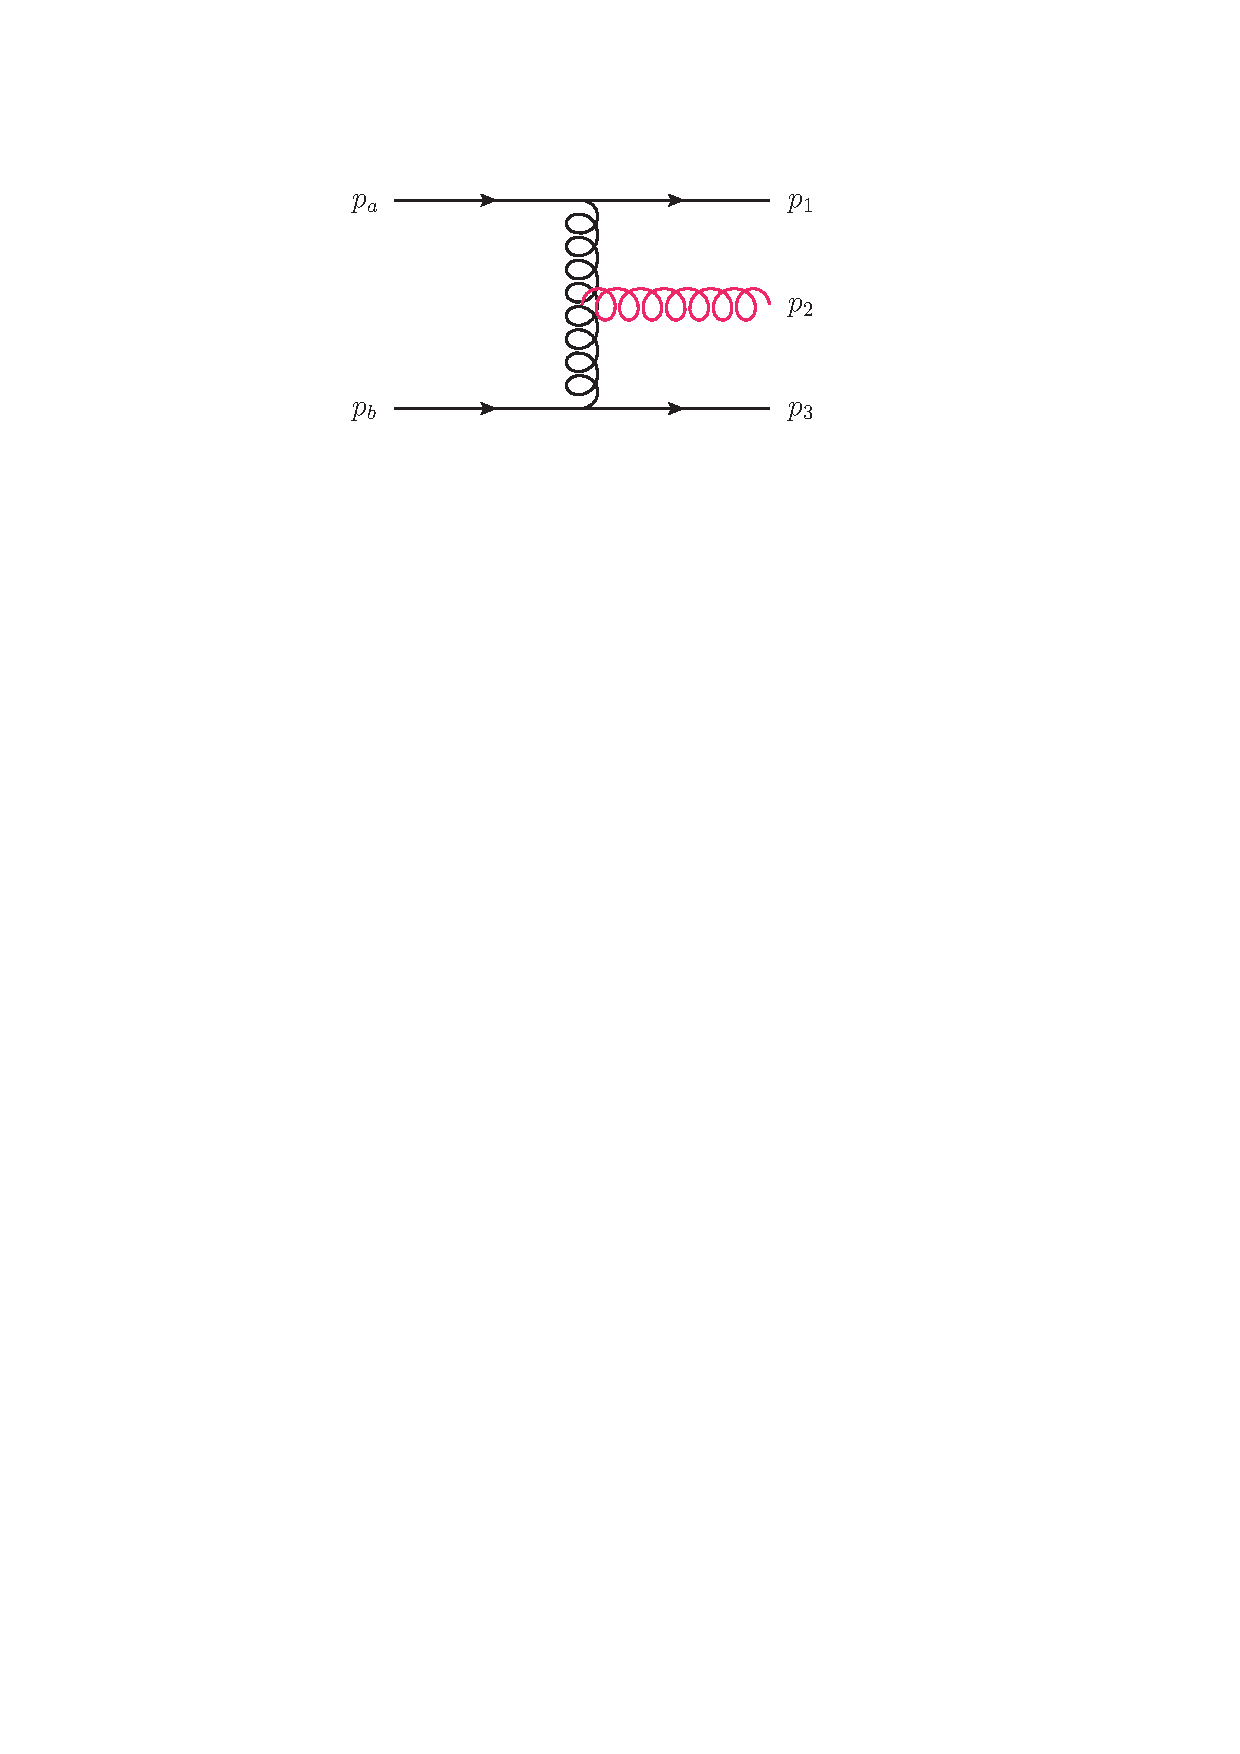
\includegraphics[scale=1]{Images/real_correction.pdf} 
\caption{If the momentum $p_2$ is small enough, we cannot detect the gluon emission and so treat it as a real correction to the $2 \to 2$ process.}
\label{fig:realcorrection}
\end{figure}

Therefore, the first real correction to $qQ \to qQ$ is
\begin{equation}
|M_{qQ \to qQ}^{HE, 1RC}|^2 = \frac{||S_{qQ \to qQ}||^2}{4 (N_c^2 - 1)}\frac{g^2 C_{F}}{\hat{t}_1} \frac{g^2 C_{F}}{\hat{t}_2} \left(\frac{4g^2 C_A}{|p_{2 \perp}|^2} \right).
\end{equation}
We need to regularise the soft divergence, so let us integrate this over the soft part of phase space (again, using dimensional regularisation) by introducing some soft transverse scale $\lambda$:
\begin{equation}
\begin{split}
& \mu^{-2 \varepsilon} \int_{soft} \frac{d^{3 + 2 \varepsilon}p_2}{(2 \pi)^{3 + 2 \varepsilon} 2E_2} \left(\frac{4g^2 C_A}{|p_{2 \perp}|^2} \right) \\
& = \mu^{-2 \varepsilon} \int_0^\lambda \frac{d^{2 + 2 \varepsilon}p_{2 \perp}}{(2 \pi)^{2 + 2 \varepsilon}} \int_{y_1}^{y_3} \frac{d y_2}{4 \pi} \left(\frac{4g^2 C_A}{|p_{2 \perp}|^2} \right) \\
&= \mu^{-2 \varepsilon} \frac{4 g^2 C_A}{(2 \pi)^{2 + 2\varepsilon}(4 \pi)} (y_3 - y_1) \int_0^\lambda \frac{d^{2 + 2 \varepsilon}p_{2\perp}}{|p_{2 \perp}|^2} \\
&= \frac{g^2 C_A}{\pi (2 \pi)^{2 + 2 \varepsilon}} (y_3 - y_1) \frac{1}{\varepsilon} \frac{\pi^{1 + \varepsilon}}{\Gamma(1 + \varepsilon)} \left( \frac{\lambda^2}{\mu^2}\right)^\varepsilon.
\end{split}
\end{equation}
By virtue of the Lipatov ansatz, the virtual corrections to the process are given by
\begin{equation}
|M_{qQ \to qQ}^{HE, VC}|^2 = \frac{||S_{qQ \to qQ}||^2}{4 (N_c^2 - 1)}\frac{g^2 C_{F}}{\hat{t}_1} \frac{g^2 C_{F}}{\hat{t}_2} \exp \left[2 \hat{\alpha}(q_{1 \perp}, \varepsilon)(y_1 - y_3) \right],
\end{equation}
and so the first virtual correction is simply the exponential expanded to first order:
\begin{equation}
\begin{split}
|M_{qQ \to qQ}^{HE, 1VC}|^2 &= \frac{||S_{qQ \to qQ}||^2}{4 (N_c^2 - 1)}\frac{g^2 C_{F}}{\hat{t}_1} \frac{g^2 C_{F}}{\hat{t}_2} \left[2 \hat{\alpha}(q_{1 \perp}, \varepsilon)(y_1 - y_3) \right] \\
& = \frac{||S_{qQ \to qQ}||^2}{4 (N_c^2 - 1)}\frac{g^2 C_{F}}{\hat{t}_1} \frac{g^2 C_{F}}{\hat{t}_2} \left[- 4 (y_3 - y_1) g^2 C_A \frac{\Gamma(1 - \varepsilon)}{(4 \pi)^{2 + \varepsilon}} \frac{1}{\varepsilon}  \left( \frac{|q_{1 \perp}|^2}{\mu^2}\right)^\varepsilon \right].
\end{split}
\end{equation}
We must now expand both of these results in $\varepsilon$, add them together and then take the limit $\varepsilon \to 0$. Doing so yields
\begin{equation}
\begin{split}
\lim_{\varepsilon \to 0} |M_{qQ \to qQ}^{HE, 1VC+1RC}|^2 &= \lim_{\varepsilon \to 0} \frac{||S_{qQ \to qQ}||^2}{4 (N_c^2 - 1)}\frac{g^2 C_{F}}{\hat{t}_1} \frac{g^2 C_{F}}{\hat{t}_2} \left[\omega_0 + \mathcal{O}(\varepsilon) \right] \\
&= \frac{||S_{qQ \to qQ}||^2}{4 (N_c^2 - 1)}\frac{g^2 C_{F}}{\hat{t}_1} \frac{g^2 C_{F}}{\hat{t}_2} \omega_0,
\end{split}
\end{equation}
with
\begin{equation}
\omega_0 = \frac{g^2 C_A}{4 \pi^2} \ln \left( \frac{\lambda^2}{|q_{1 \perp}|^2}\right).
\label{eqn:omega}
\end{equation}
The argument clearly continues to higher orders and so we can immediately generalise the result to yield a full HEJ amplitude:
\begin{equation}
\begin{split}
|M_{f_1f_2 \to f_1...f_2}^{HEJ}|^2 &= \frac{||S_{f_1 f_2 \to f_1 f_2}||^2}{4 (N_c^2 - 1)}\frac{g^2 C_{f_1}}{\hat{t}_1} \frac{g^2 C_{f_2}}{\hat{t}_{n-1}} \\
& \prod_{i=1}^{n-2} \frac{-g^2 C_A V(q_{i}, q_{i+1}) \cdot V(q_{i}, q_{i+1})}{\hat{t}_{i} \hat{t}_{i+1}}  \\
& \prod_{j =1}^{n-1} \exp \left[ \omega_0(q_{j \perp})(y_{j+1} - y_j) \right].
\end{split}
\label{eqn:fklresum}
\end{equation}
The final comment to make about the HEJ amplitude is that we can extend it to also include the emission of a Higgs \cite{Andersen2011a}, a $W^{\pm}$ \cite{Andersen2012} or a $Z$ boson \cite{Andersen2016} along with the jets. The only difference is the form of the current contraction $S_{f_1f_2 \to f_1 f_2}$. For the pure jets case, this is simply $j_\mu j^\mu$, the contraction of two pure quark currents. We can also define a current for the emission of, for example, a $W$ boson as $j^\mu_W$, which will depend on the momenta of the decay products of the $W$ along with the momentum of the quark line. For a $W$ process, then, we would have an object $S_{f_1 f_2 \to f_1 f_2 e \nu} = j^\mu_W j_\mu$. The rest of the derivation then proceeds as before. 

\section{Monte Carlo Implementation}

We now have an expression for an all-order matrix element that is free of divergences in four spacetime dimensions. For physical relevance, we must now integrate the matrix element over the entire detector phase space of the LHC. The general expression for the integrand has already been shown in section 1.5. The way we do this complicated integral is via the technique of \emph{Monte Carlo Integration} and we dedicate this section to explaining the process within the context of our implementation.

\subsection{The Motivation Behind Monte Carlo}
Monte Carlo integration is a numerical integration technique that provides an estimate for a (usually very complicated or even analytically undoable) integral via use of random numbers. An insightful example of how it works is to consider how it can be used to estimate the value of $\pi$. Figure \ref{fig:estpi} shows a simple setup for how to achieve this. The area of the blue square is $(2R)^2$ and the area of the red circle is $\pi R^2$. The ratio of the area of the circle to the area of the square is then $\pi/4$. If we were to pick a random point in the square (since we have only two dimensions here, this is the same as randomly sampling a pair of $x$ and $y$ coordinates) then there is a probability of $\pi/4$ that it also falls within the circle. Therefore, given $N$ total choices of points within the square (or `trials') of which $M$ also fall inside the circle,
\begin{equation}
\pi \approx \frac{4M}{N}.
\end{equation} 
Of course, if we do not conduct many trials $N$, our approximation will not be a good one because we have simply not sampled enough of the available space. As we increase our number of trials, however, the approximation gets closer to the real value of $\pi$, as shown\footnote{In fact, we tend to `bounce' around the true value of $\pi$ because the nature of our approximation means we constantly switch between overestimating and underestimating the true value.} in table \ref{tab:estpi}. This is a consequence of the \emph{law of large numbers}, on which Monte Carlo techniques depend. 

\begin{figure}[t]
\centering
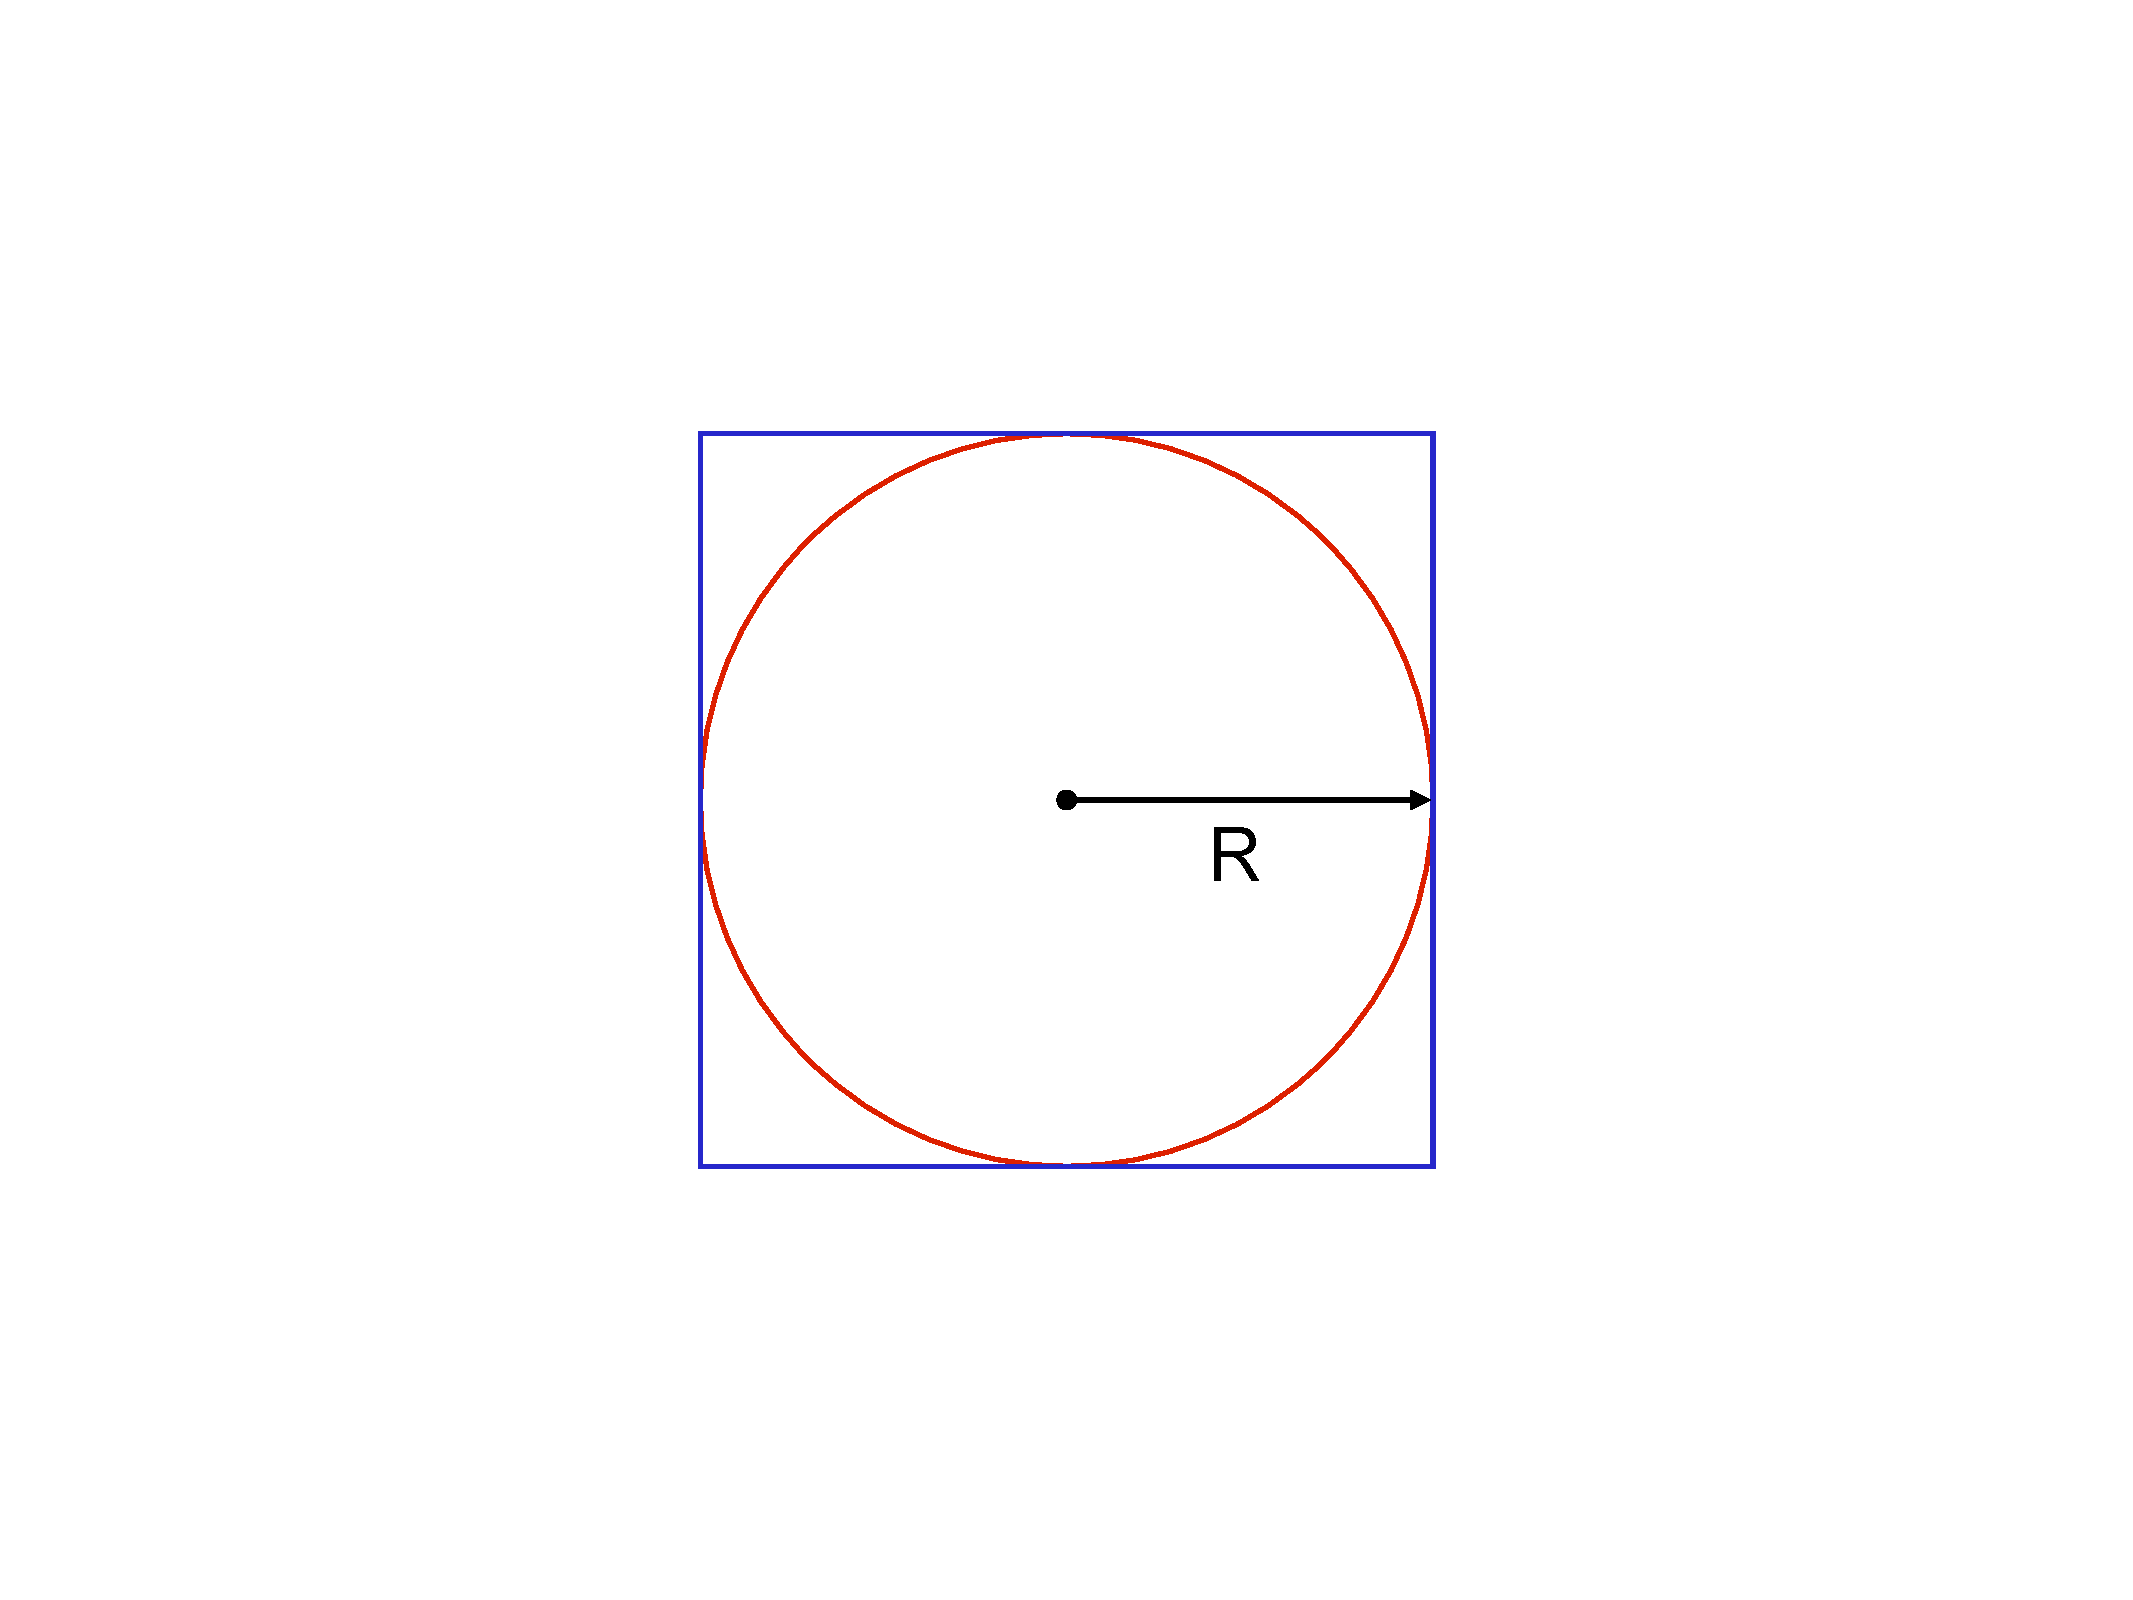
\includegraphics[scale=0.5]{Images/monte_carlo.pdf} 
\caption{A square with sides of length $2R$ enclosing a circle of radius $R$. We can estimate the value of $\pi$ by picking random points in the square and seeing whether or not they also lie in the circle.}
\label{fig:estpi}
\end{figure}

\begin{table}[t]
  \centering
  \begin{tabular}{ | m{5cm} | m{5cm} | }
    \hline
    \centering Number of trials & Estimate of $\pi$ \\ \hline
    \centering $10^0$
    & 
    4
    \\ 
    \centering $10^1$
    & 
     2
    \\ 
    \centering $10^2$
    & 
    3.6
    \\ 
    \centering $10^3$
    & 
    3.192
    \\
    \centering $10^4$
    & 
    3.1644
    \\
    \centering $10^5$
    & 
    3.1404
    \\
    \centering $10^6$
    & 
    3.141828
    \\
    \centering $10^7$
    & 
    3.14139320
    \\
    \centering $10^8$
    & 
    3.14145576
    \\
    \centering $10^9$
    & 
    3.14161324
    \\                   
    \hline
  \end{tabular}
  
  \caption{Estimates of $\pi$ via a simple Python Monte Carlo program for different numbers of trials.}
  \label{tab:estpi}
\end{table}

To make clear the relation to integral problems, we will discuss this problem again from a different point of view. We can think of the square which contains the circle as a two-dimensional `volume' (more usually called area, of course, but we will introduce the more general term now) which bounds our system with value $V_2 = 4 R^2$. Within this volume, we are trying to calculate another volume; namely, the area of the circle. Taking the origin of our co-ordinate system to be the centre of the circle, then the area of the circle is given by
\begin{equation}
V_C = \int_0^R dr \hspace{2pt} r \int_0^{2 \pi} d \theta \equiv \int_{V_C} d \Omega.
\end{equation}
This is a particularly simple integral with value $V_C = \pi R^2$. In the initial formulation of the problem, we took this to be known but were ignorant on what the value of $\pi$ numerically is. Instead, let us imagine that we did not know how to perform the integral at all. We always know, however, that an integral (which we generalise to one depending on many variables) can be related to the average value of its integrand:
\begin{equation}
\left< f(\vec{x}) \right>_{x \in V} = \frac{\int_V d \Omega f(\vec{x})}{V}.
\end{equation}
The average can be estimated by simply sampling the integrand at $N$ random points and then dividing by $N$. So long as the distribution of random points in the volume is flat, the \emph{Central Limit Theorem} guarantees that
\begin{equation}
\int_V f(\vec{x}) d \Omega \approx V \left<f \right> \pm V \sqrt{\frac{\left<f^2 \right> - \left<f \right>^2}{N}},
\label{eqn:mcmaster}
\end{equation}
with
\begin{subequations}
\begin{align}
\left<f \right> &= \frac{1}{N} \sum_{i=1}^{N} f(\vec{x_i}), \\
\left<f^2 \right> &= \frac{1}{N} \sum_{i=1}^{N} f^2(\vec{x_i}).
\end{align}
\end{subequations}
It is important to note that the error estimate here assumes the error is distributed in a Gaussian fashion. We clearly see that it scales as $N^{-\frac{1}{2}}$, which is rather slowly convergent, but the important point is that it is \emph{completely independent of the dimensionality} of the problem.  

The last step is to increase the domain of integration to the larger area $V_2$ that encapsulates entirely $V_C$:
\begin{equation}
\int_{V_C} d \Omega \hspace{2pt} f  = \int_{V_2} d \Omega \hspace{2pt} f|_{V_C} \approx V_2 \left< f|_{V_C}  \right> \pm V_2 \sqrt{\frac{\left< f|_{V_C} ^2 \right> - \left< f|_{V_C}  \right>^2}{N}}.
\end{equation}
Then, since in our original problem the integral we are interested in is simply the area integral, $f = 1$ if any chosen random point is within $V_C$ and $0$ otherwise. Thus, given $N$ trials of which $M$ lie inside the circle (we drop the error estimate now for brevity),
\begin{equation}
\begin{split}
\int_{V_2} d \Omega \hspace{2pt} 1|_{V_C} = V_C \approx V_2 \frac{M}{N} \\
\therefore \frac{V_C}{V_2} \approx \frac{M}{N},
\end{split}
\end{equation}
which is the statement we started with. 

We could imagine extending this experiment in two ways. Firstly, we could be interested in the behaviour of a more complicated function within a volume (i.e., a more complicated $f$). Secondly, we could also think about taking the problem into three dimensions by considering a sphere enclosed within a cube. Indeed, mathematically speaking, we could extend this into as many dimensions as we desire, to the point where we no longer have such an obvious geometric interpretation of the problem. It is precisely the arena of high-dimensionality integration problems with complicated integrands where Monte Carlo techniques come into their own.

\subsection{Monte Carlo in High Energy Jets}

We recall from section 1.5 that the integral we are trying to perform looks like
\begin{equation}
\sigma_{pp \to n-jet}^{inc/exc} = \sum_{f_a, f_b} \int_0^1 dx_a \int_0^1 dx_b f_a(x_a, Q^2) f_b(x_b, Q^2) \times \hat{\sigma}_{partonic} \times \mathcal{J}(\text{n-jet}^{inc/exc}),
\end{equation}
with
\begin{equation}
\hat{\sigma}_{partonic} = S \times \frac{|M|^2}{F} \times (2 \pi)^4 \delta^{(4)}(p_a + p_b - \sum_{f=1}^n p_f) \times \prod_{i=1}^n \int \frac{d^3 \vec{p}_i}{2 E_i (2 \pi)^3},
\end{equation}
and so the problem is clearly suited to evaluation by Monte Carlo methods. The general process is as follows:

\begin{enumerate} 
\item{Generate a number of partons for the final state.}
\item{Pick the flavours for the incoming state.}
\item{Generate the momenta for all partons.}
\item{Perform a basic cluster into jets to check whether this event will give something consistent with cuts (a set of kinematical constraints imposed on the analysis). If not, throw away the point here and start again.}
\item{Calculate the matrix element and multiply by other factors in the integrand.}
\item{Cluster into jets and check to see if they pass all imposed cuts on the process. If it does, add the calculated point to the estimation of the average.}
\item{Repeat.}

\end{enumerate}

Such a technique is perfectly acceptable and results can be achieved this way. However, if we are simply generating random numbers flatly in these steps then we are being needlessly inefficient. For example, we see from graphs of Parton Distribution Functions that there are clear areas where the value of it is much larger than at other points. If we simply generate flatly then we equally sample these two regions which will clearly hurt our convergence. Indeed, there is a technique to combat this called \emph{importance sampling}. 

Importance sampling is aimed at reducing as much as possible the value of $\sqrt{\left<f \right>^2 - \left<f^2 \right>} \equiv \sigma_{MC}$, also known as the \emph{variance}, which we saw was directly related to the estimate of the error. To see how this achieved, let us consider a one-dimensional integral and utilise our freedom to multiply and divide by another (well-behaved) distribution $q(x)$:
\begin{equation}
\int_a^b dx f(x) = \int_a^b dx \hspace{2pt} q(x) \frac{f(x)}{q(x)} = \int_a^b dx \hspace{2pt} q(x) h(x).
\end{equation}
We can then perform a change of variables
\begin{equation}
\int_a^b dx \hspace{2pt} q(x) h(x) = \int_{Q(a)}^{Q(b)} dy \hspace{2pt} h \left(Q^{(-1)}(y) \right),
\end{equation}
with $dQ(x)/dx = q(x)$. If we normalise $q(x)$ such that it integrates to unity over the integration domain, then the fundamental theorem for Monte Carlo integration shows
\begin{equation}
\int_a^b dx f(x) = \int_a^b dx \hspace{1pt} q(x) \frac{f(x)}{q(x)} \approx \left< \frac{f(x)}{q(x)} \right> \pm \sqrt{\frac{\left<f^2(x)/q^2(x)\right> - \left<f(x)/q(x) \right>^2}{N}}.
\end{equation} 
Thus if we pick $q(x) = 1/(b-a)$, we arrive back at equation \ref{eqn:mcmaster} (a one-dimensional volume is simply the length of the line), but we are not bound to make this choice -- we should instead pick a $q(x)$ that minimises as much as possible the second term. There are a few subtleties and difficulties in doing this, but the upshot is that this is best achieved by sampling from a distribution $q(x)$ that is close to $f(x)$ in shape. This is done at many points in the HEJ program, including:

\begin{itemize} 
\item{Picking the incoming partons in such a way to more often sample those with a higher PDF value. The LHAPDF package \cite{Buckley2014} which contains a whole range of different PDF sets to choose from provides the value of $f/x$, so what we actually optimise for is the quantity $x \times f/x$.}
\item{Generating transverse momenta skewed towards the lower end of the spectrum since the cross-section falls off rapidly with $p_\perp$.}
\item{Generating the rapidity of particles to more often create `valid' configurations, where we keep the FKL rapidity ordering.}
\end{itemize}

With such considerations, the variance of our estimate is greatly reduced and stable results can be obtained fairly quickly, depending on the precise nature of the analysis. 

\subsection{Concerning Partons and Jets}
In the previous subsection it was remarked that during our Monte Carlo program we check to see how the partons we generate correspond to observed jets. How this is done is worthy of a longer discussion. The process by which hard partons produced by the scattering culminate in jets of hadrons is an inherently non-perturbative process; there is no such effect that arises naturally from the rules of our perturbation theory. The implication is clear: perturbation theory must break down at some point. The cause of this is that the value of the expansion parameter $\alpha_s$ is not a constant but `runs' with the energy scale as shown in figure \ref{fig:alphas}. At small energy scales, the parameter becomes large enough that a perturbative theory no longer makes sense. Thankfully, we can separate (or `factorise') these low energy processes away from our high energy perturbative process so long as we have a defined way of estimating how many final state jets appear given a certain set of hard external partons. This has led to the development of \emph{jet algorithms}. 

\begin{figure}[t]
\centering
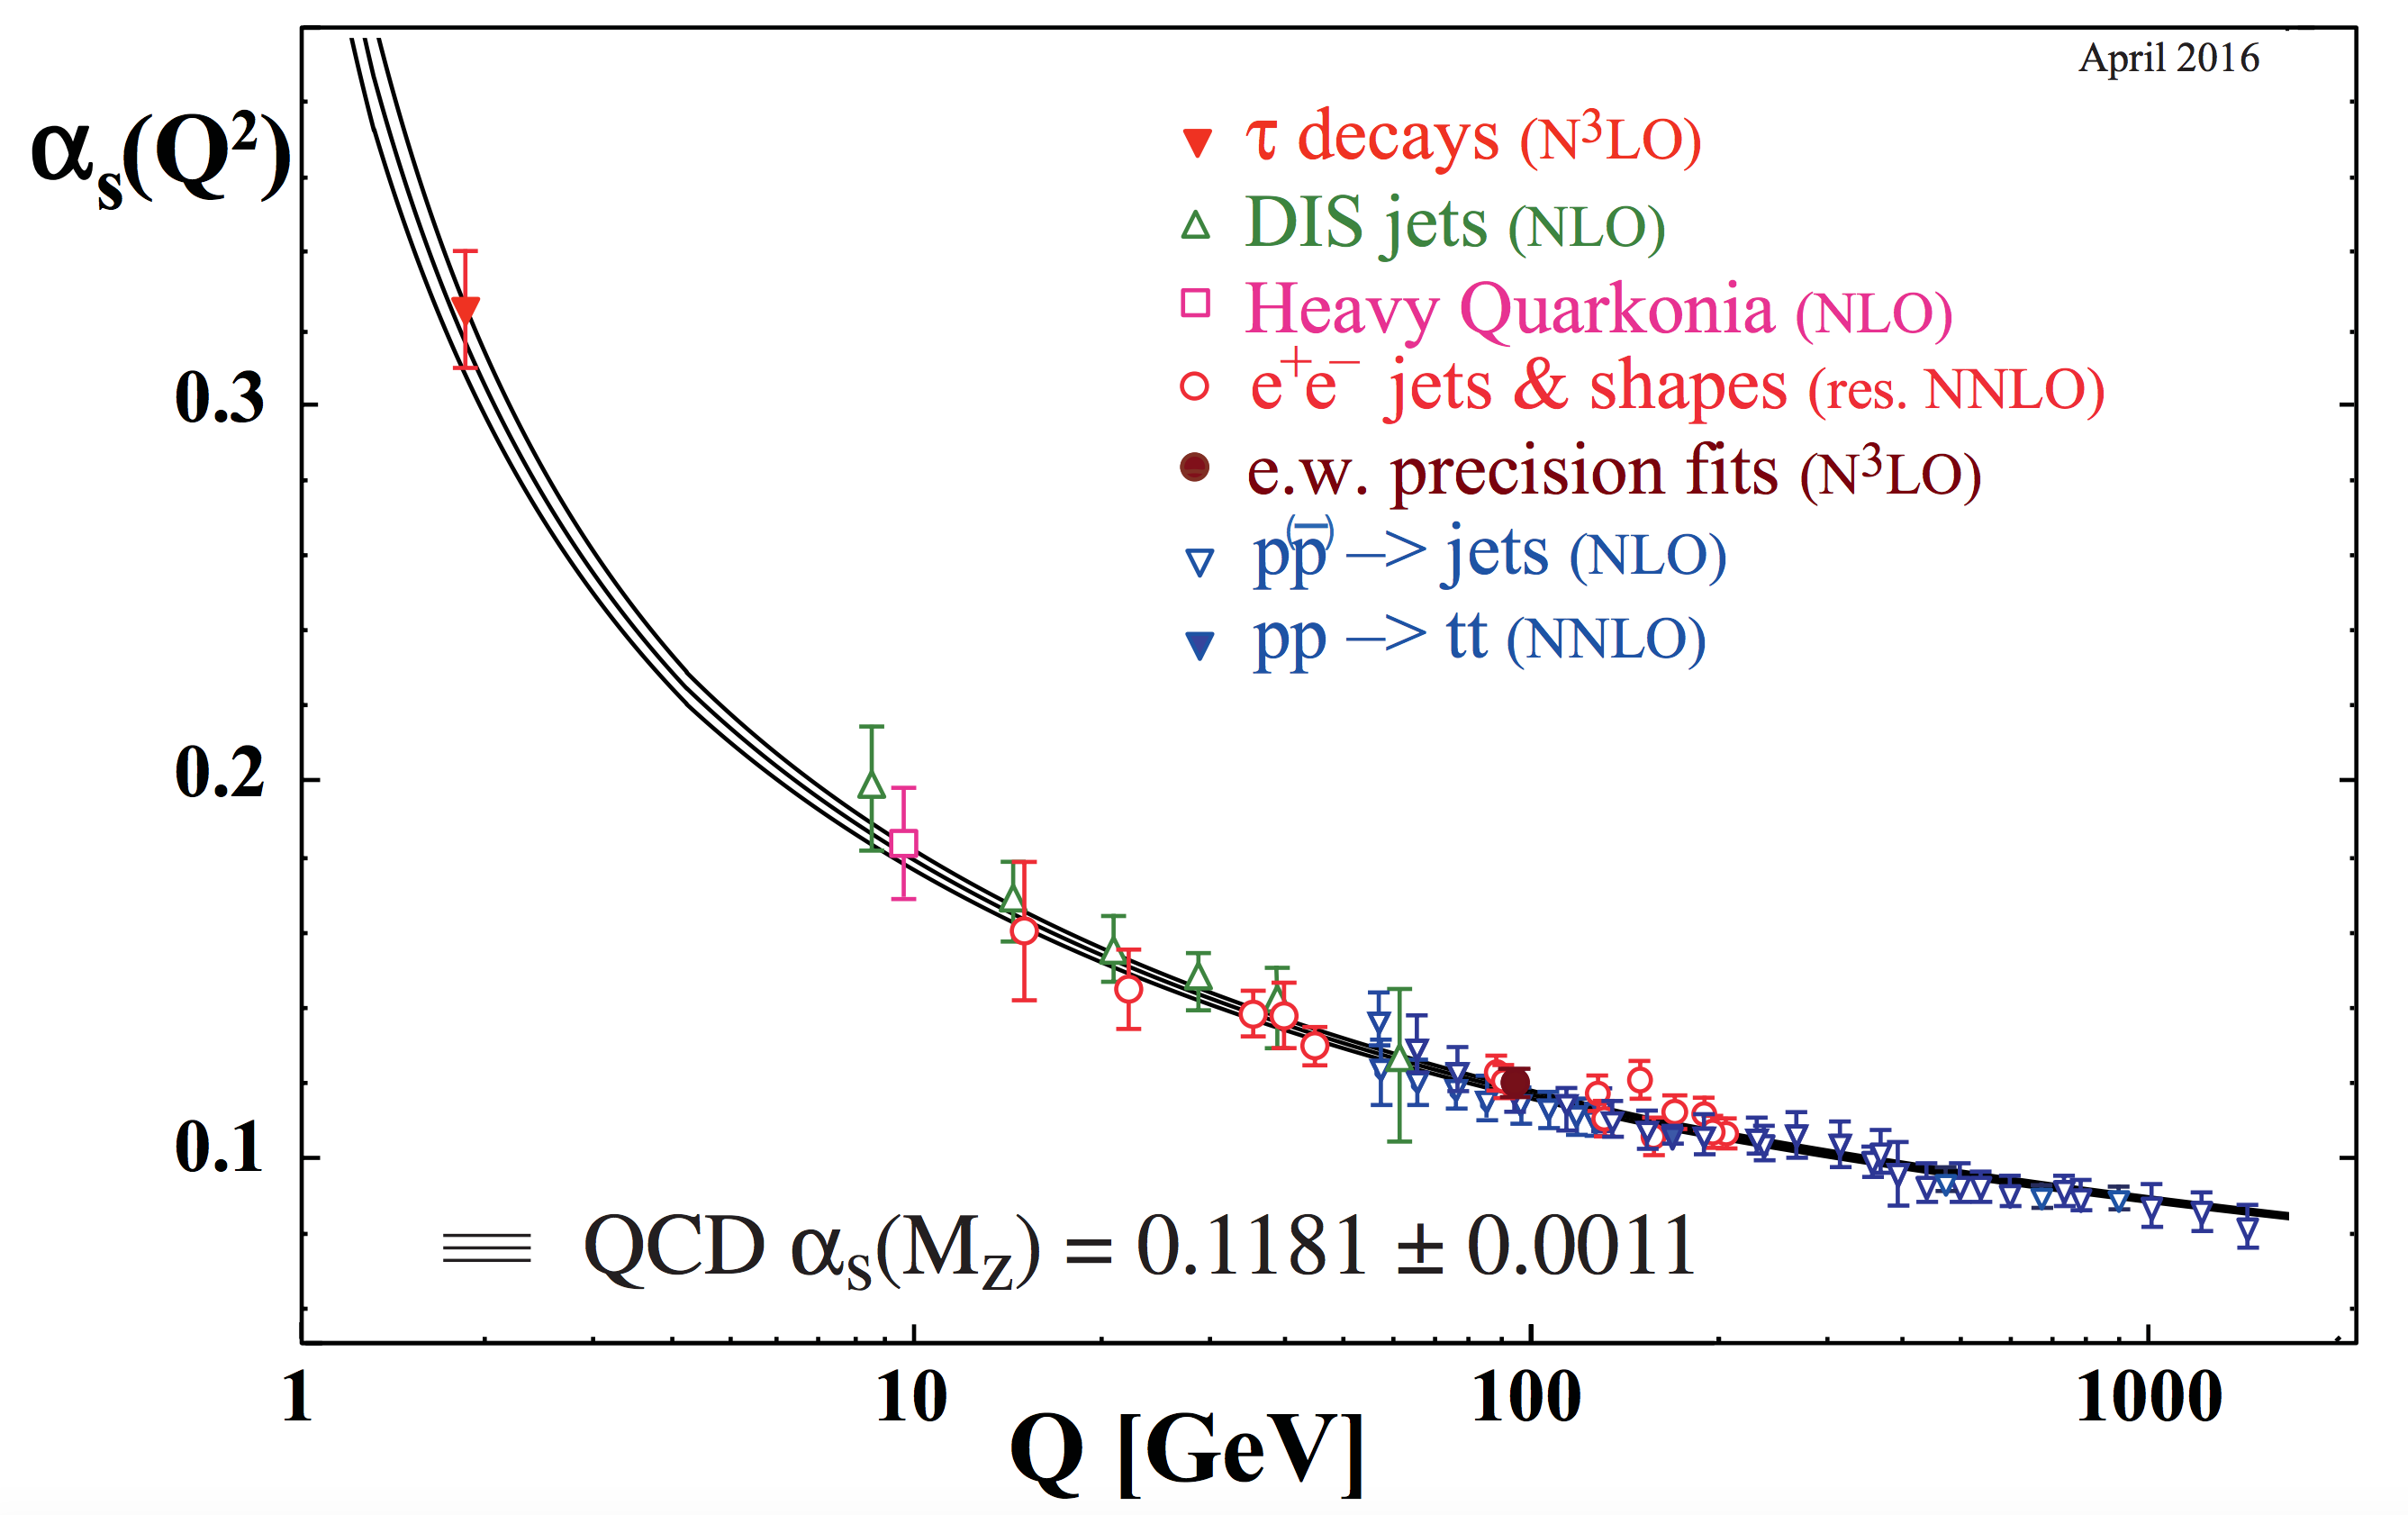
\includegraphics[scale=0.3]{Images/running_alphas.png} 
\caption{The value of $\alpha_s$ as evaluated at different energy scales $Q^2$. At low energies, the value becomes large enough that a perturbative treatment of QCD is no longer valid. Taken from \cite{Hagiwara2002}.}
\label{fig:alphas}
\end{figure}

There are two broad categories of algorithms: `Cone-Type' and `Sequential Clustering' \cite{Atkin2015}. The first type are heavily disfavoured by the theory community because of their tendency to be infrared unsafe (meaning they depend on the low energy physics of the underlying theory) and so we will focus on the second type. The general process for this type of algorithm is as follows:

\begin{enumerate}
\item{Define some distance measure $d_{ij}$ that can be calculated between each pair of hard partons $i,j$ and a distance $d_{iB}$ between all particles and the beam line.}
\item{Compute all distances $d_{ij}$ and $d_{iB}$ and find the smallest.}
\item{If the smallest distance is a $d_{ij}$, then combine the momenta of the partons $i, j$ and recalculate all distances. If the smallest is a $d_{iB}$, remove parton $i$ from the process and call it a `jet'.}
\item{Repeat until all partons are clustered into jets.}
\end{enumerate}

The natural question, of course, is what we should choose for the distances $d_{ij}$ and $d_{iB}$. The general form is
\begin{equation}
\begin{split}
d_{ij} &= \text{min}\left(k_{i \perp}^{2p},k_{j \perp}^{2p} \right) \frac{\Delta_{ij}}{R} \hspace{10pt} \text{with} \hspace{10pt} \Delta_{ij} = \sqrt{(y_i - y_j)^2 - (\phi_i - \phi_j)^2} \\
d_{iB} &= k_{i \perp}^{2p}.
\end{split}
\end{equation}
The parameter $R$ scales the $d_{ij}$ with respect to $d_{iB}$ such that any pair of final jets $a, b$ are at least separated by $\Delta_{ab} = R$. For this reason, we often refer to $R$ as a `jet radius'. The value of $p$ can be chosen to govern the relative power of energy and geometrical scales in the distance parameter. There are three main algorithms which have three different choices for $p$: the kT algorithm with $p =1$, the Cambridge/Aachen with $p=0$ and the anti-kT with $p = -1$ \cite{Atkin2015}. There are reasons why one might want to use one over the other and so one would wish for a simple way of changing between conventions in any computer program one wants to run. Fortunately, the \emph{FastJet} library \cite{Cacciari2012} does precisely this. For the user, the only requirement is to specify which algorithm is to be used at the start of the calculation. Any further calculations involving the jet objects are easily handled within the defined classes in the package. 

\subsection{Scale Variations}

It has already been discussed that the value of a parton distribution function is dependent on the energy scale at which the proton is probed. We have now seen that the value of the strong coupling constant $\alpha_s$ is also dependent on the energy scale. In principle, these two scales are different, and called the \emph{factorisation scale} $\mu_f$ and \emph{renormalisation scale} $\mu_r$ respectively. Clearly, we need to make a choice for these scales before we can do any calculations. However, it is not clear at all what we should choose. We can imagine at least that the scales do not differ much and so we could simply consider $\mu_f = \mu_r$. Still, we find there is no one good answer to this question and we are left with the task of calculating \emph{scale variations} in order to provide an estimate of uncertainty to our calculation arising from this. With HEJ, we by default allow for the input of four different scale choices: 

\begin{enumerate}
\item{Fixed scale;}
\item{Maximum jet $p_\perp$;}
\item{$H_T/2$, which is the scalar sum of all parton $p_\perp$ divided by 2;}
\item{Invariant mass of the jets.}
\end{enumerate} 

When calculating scale variations, we take the scale as defined and then vary independently $\mu_f$ and $\mu_r$ around it by factors of $2, \sqrt{2}, 1, \frac{1}{\sqrt{2}}, \frac{1}{2}$. Since there are five choices for each scale, we overall have 25 different results. However, since we expect $\mu_f$ and $\mu_r$ to be close to each other, we remove the points where $\mu_f/\mu_r > \sqrt{2}$ or $\mu_r/\mu_f > \sqrt{2}$, which leaves us with 19 options. These will form bands around a central prediction, which we then use as our estimation for the effect of scale variation for our results. %\todo{Explain how this might be improved}

\section{Experimental Analyses}

We have spent the best part of this chapter arguing from a theoretical standpoint that the systematic treatment of High Energy logarithms is required for the accurate description of LHC data. We would like to end this chapter by providing plots from actual LHC analyses to show that the experimental data actually agrees with that statement. HEJ has been used in a wide range of experimental analyses \cite{Aad2011, Chatrchyan2012, Chatrchyan2012a,Abazov2013,Aad2014a,Aad2014,Aad2015} and we present a few select plots for discussion here. To understand them all fully, we first need to explain a couple of other features of HEJ we have not yet presented. 

Firstly, HEJ includes a multiplicative matching to full LO calculations for matrix elements up to and including four final state jets. After a process has been clustered into final state jets, the matrix element is recalculated with the jet momenta\footnote{Since some partons may not make it into final state jets, momentum conservation may not necessarily hold here. This is solved by distributing the momenta of partons that are not included into the jets in such a way as to keep it as close as possible to the original jet momenta.} along with the full LO matrix element (currently provided by \emph{MadGraph} \cite{Alwall2011}) and the process is multiplied by the ratio of the full LO result to our matrix element. We also include full LO matrix elements for non-FKL processes, which we saw are sub-leading in the high energy limit but important in other regions of phase space. Including matching in this way allows HEJ to be as competitive as other approaches in areas far away from the high energy limit it is designed for. 

Secondly, it is possible to interface HEJ with the \emph{parton shower} ARIADNE \cite{Andersen2011}. A parton shower is designed to simulate the hadronisation of the event and as such is a completely distinct problem from that of calculating the hard scattering matrix element that HEJ provides. The specifics of the technique are interesting \cite{Hoche2014} but beyond the scope of this thesis. The important point is that a combined HEJ+ARIADNE program can describe the high energy behaviour of the hard scattering element along with the soft behaviour of the parton shower. 

\begin{figure}[t]
\centering
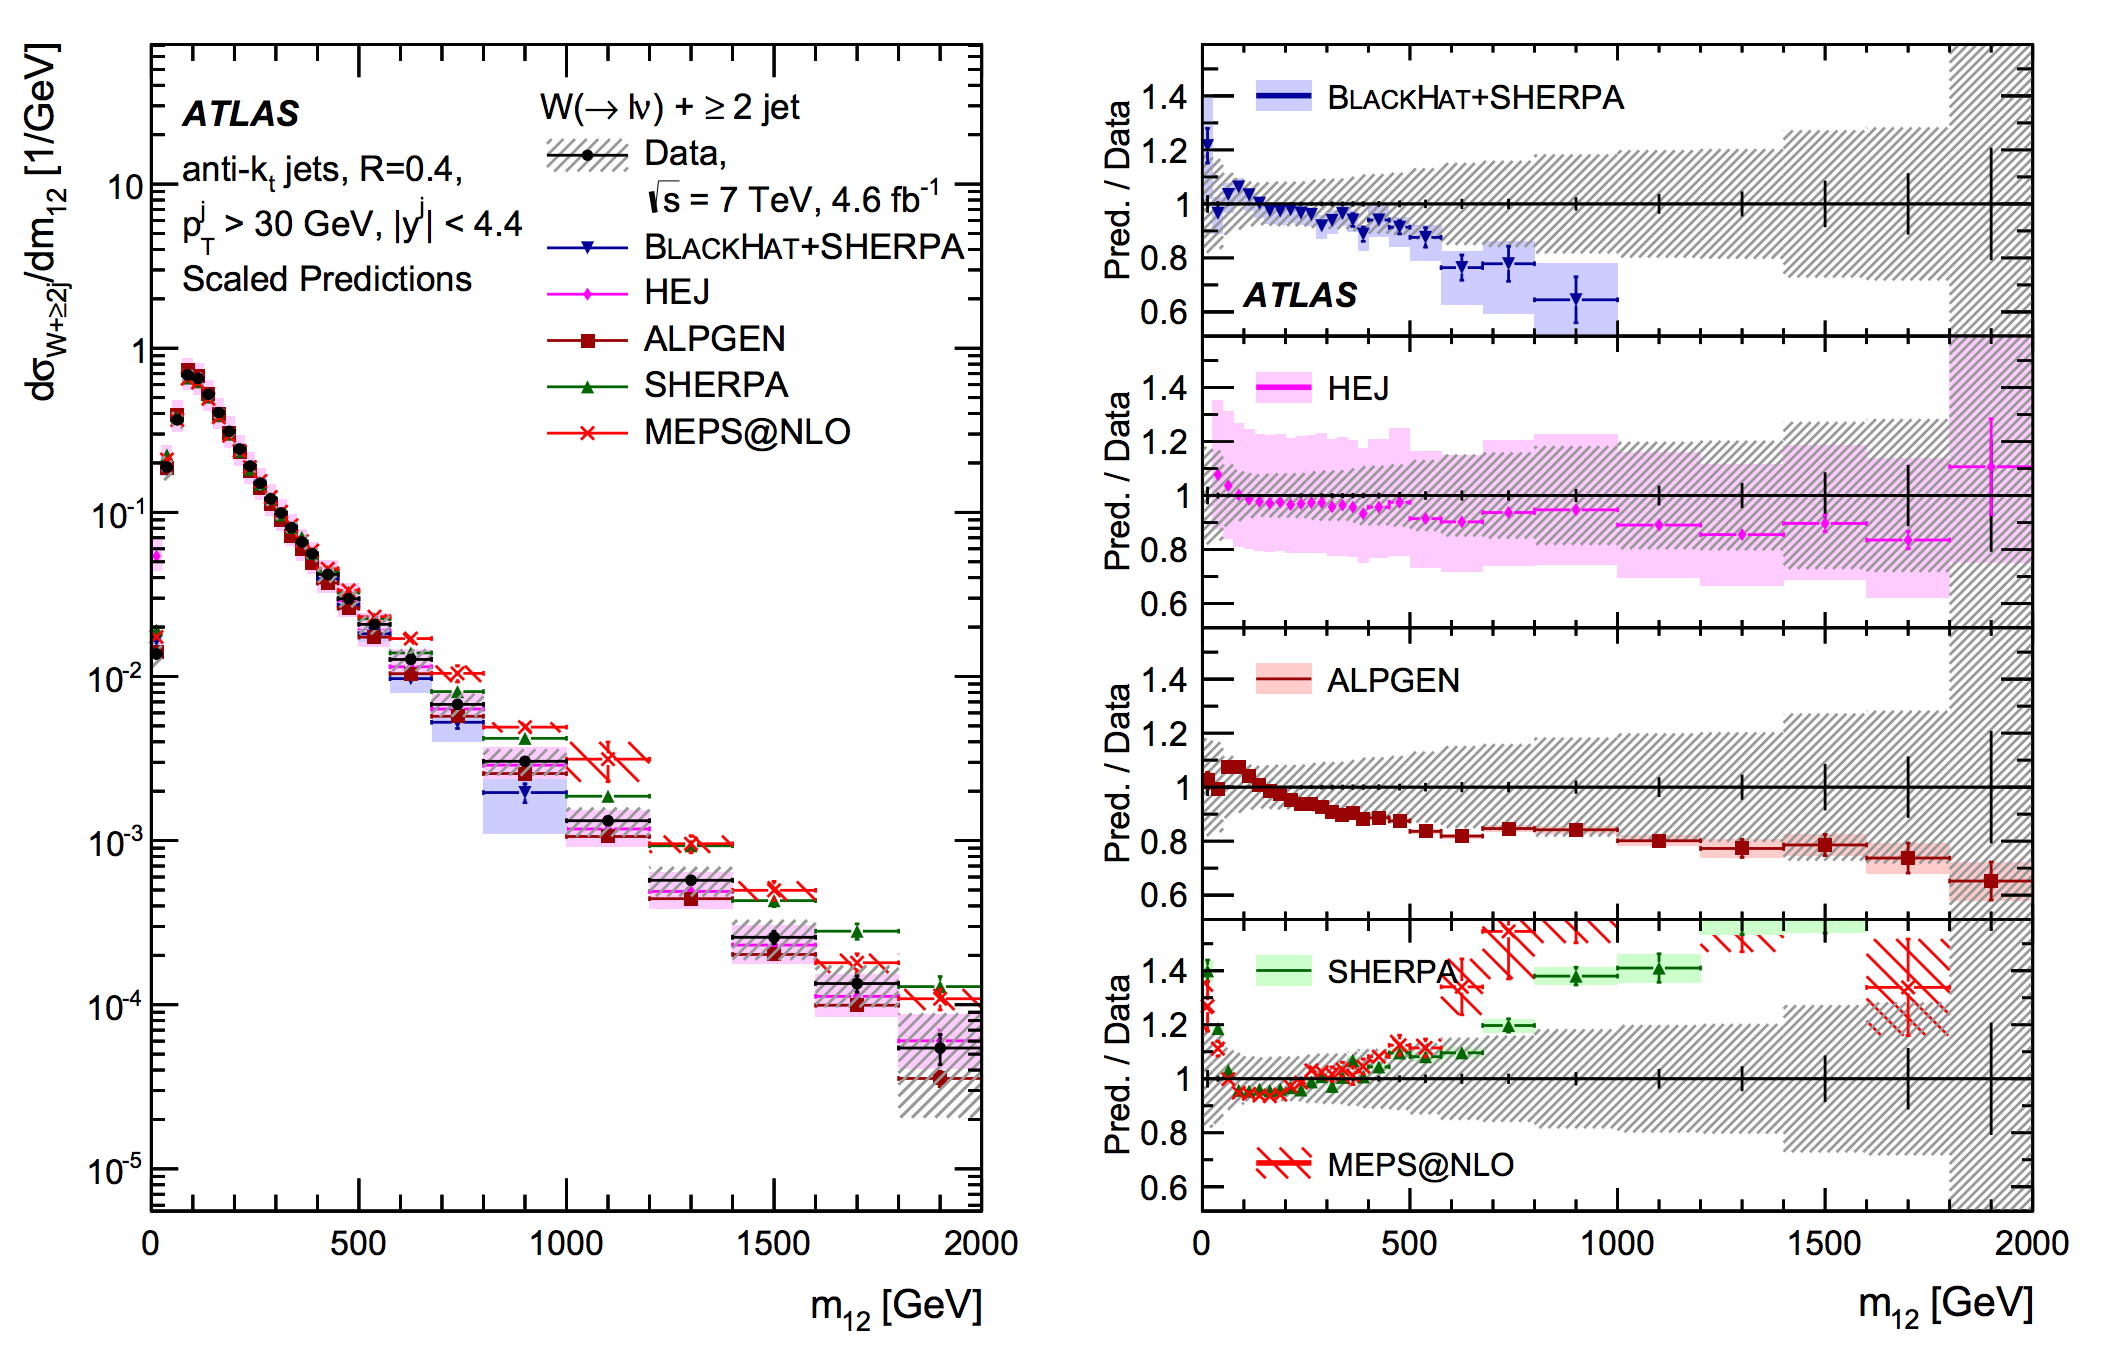
\includegraphics[scale=0.4]{Images/wjets_HEJ.png} 
\caption{Differential cross-section in $m_{12}$ bins in the ATLAS study \cite{Aad2014a}}
\label{fig:wjet}
\end{figure} 
%\todo{The last one looks shit}

Figure \ref{fig:wjet} shows a range of predictions for a $W$ plus at least two jet event, binned in the invariant mass between the most forward and backward jet. The tail of this distribution is precisely where we expect the high energy logarithms to become important. The failure of the fixed order approaches to describe this region well clearly shows that this is indeed the case. The error band on the HEJ prediction is large and comes from the scale variations; the scale variation bands are not included on the other generators in the plot and would be just as large. The exception is the BlackHat line: their scale variation is shown and it is smaller than HEJ's because it is an NLO calculation, whereas HEJ only matches to LO. It is clear from the flatness of HEJ's line in the ratio plot that it is the only prediction tracking the data. Indeed, further investigation in \cite{Andersen2016} showed that the scale variation has the effect of an overall normalisation and has no bearing on the shape.  

\begin{figure}[t]
\centering
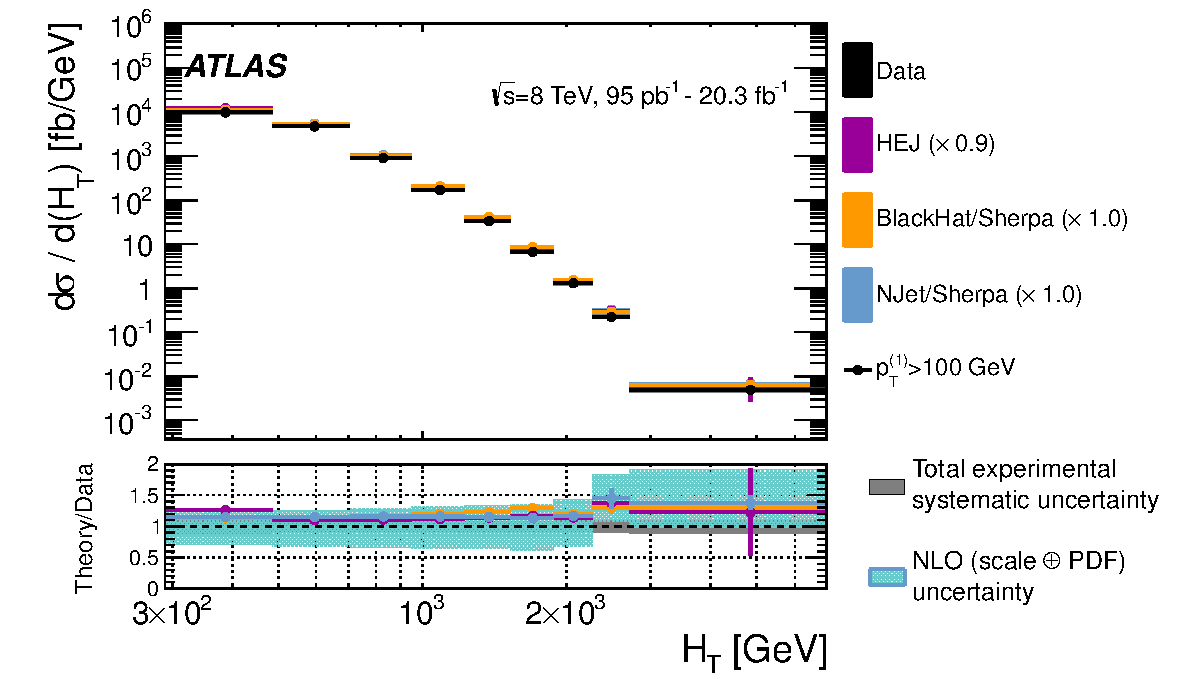
\includegraphics[scale=0.8]{Images/4jet_hej.pdf} 
\caption{Differential cross-section in HT (the scalar sum of all jet momenta) bins in a four jet ATLAS study \cite{Aad2015}.}
\label{fig:4jetan}
\end{figure}

Figure \ref{fig:4jetan} shows the cross-section for a process involving at least four final state jets binned in $H_T$, which is the scalar sum of all transverse momenta. The interesting feature of this plot is that HEJ continues to match the data out to high values of $H_T$, which correspondingly means high values of $p_\perp$ for (at least one of) the jets. The High Energy Limit that inspired HEJ holds only when the $p_\perp$ of the final state particles are all much smaller than the centre of mass energy and therefore should not be expected to provide a good description in the regime probed here. We see that HEJ keeps enough of the full process and this, along with the matching procedure, allows for it to be a fully completive description in a large part of the LHC phase space. 

\begin{figure}[t]
\centering
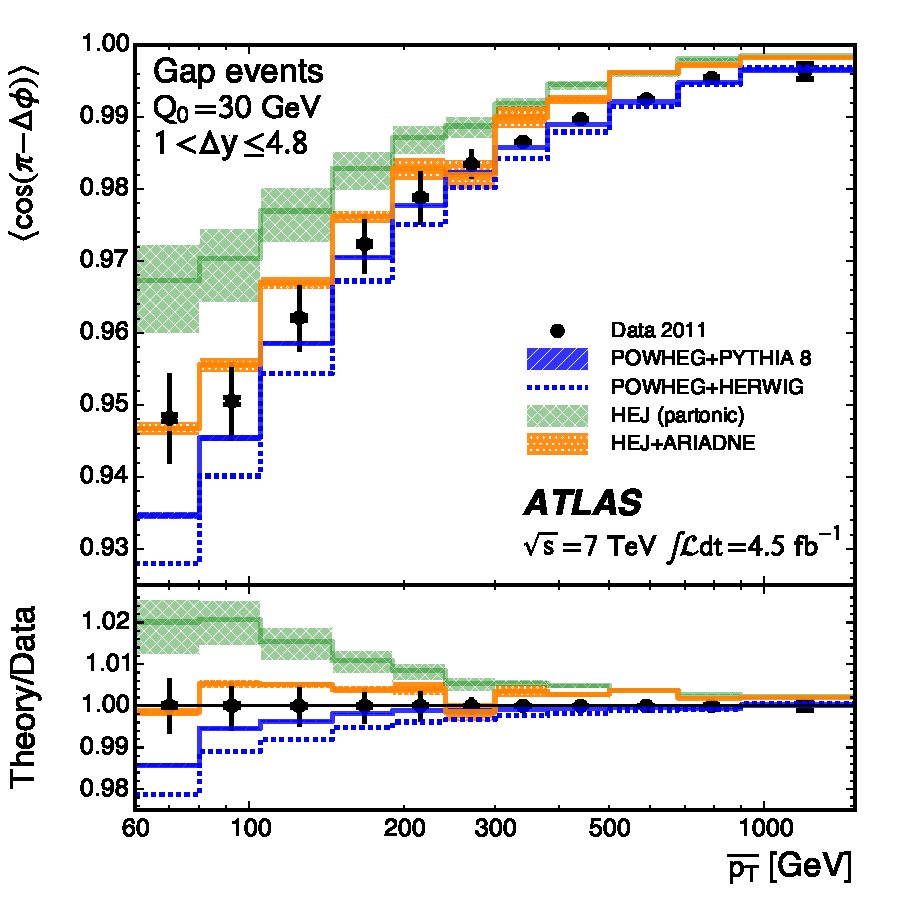
\includegraphics[scale=0.8]{Images/hej_powheg_agree.pdf} 
\caption{Plot of an azimuthal decorrelation observable in average $p_\perp$ in the ATLAS analysis \cite{Aad2014}.}
\label{fig:vetoptbar}
\end{figure}

Figure \ref{fig:vetoptbar} is a plot from an analysis involving a jet veto. A scale (in this case, 30 GeV) is chosen whereby any extra jet emission in a rapidity gap between a defined two-jet system (here, the most forward and backward jets) is vetoed. Such a measurement is useful for testing perturbative predictions on the absence of activity in the gap; for example, we see from our HEJ amplitude that a large $\Delta y$ corresponds to a larger value of the resummation exponential. The predictions for both HEJ and HEJ+ARIADNE are shown for an observable related to the angular decorrelation of the dijet system. It is clear in this case that the best description of data comes from having both the high energy and the parton shower effects included; in the first few bins the partonic HEJ, which only includes the former, overshoots, and the POWHEG line, which only includes the latter, undershoots. The orange line (HEJ + ARIADNE), containing both, tracks the data excellently. 

All of these analyses were performed during the first run of the LHC with a centre-of-mass energy of either 7 or 8 TeV. Run II will provide us with data for events at a centre of mass energy of 13 or 14 TeV and so we expect that the effect of these high energy logarithms will become even more prevalent in future analyses. 
